%スライド用コマンド-dvipdfmじゃないと栞は作られない
\documentclass[dvipdfmx,graphicx,14pt]{beamer}
%\usepackage{etex} % In order to use too many packages
%\documentclass[dvipdfmx,graphicx]{beamer}
%handout用コマンド
%パワポと同じ事をしたいとき
%\documentclass[8,9,10,11,12,14,17,20pt, dvips, handout]{beamer}
%\documentclass[compress,dvipdfm,handout]{beamer}
%文書を作りたいとき
%\documentclass[a4paper,12pt,dvipdfm]{jarticle}
%\usepackage{beamerarticle}

\usepackage{my_slide}
%\useoutertheme[subsection=false]{smoothbars}
%\setbeamertemplate{footline}[page number]
\setbeamerfont{footline}{size=\small,series=\bfseries}
\setbeamercolor{footline}{fg=black,bg=black}
\usepackage{appendixnumberbeamer}
\setbeamertemplate{section in toc}[sections numbered]

\usepackage{my_math_macros}

\usepackage{color}
\usepackage{url}
\usepackage{tikz,tikz-3dplot}
\usetikzlibrary{dsp,positioning,calc,backgrounds}
\usepackage{amsthm}

% 日本語をゴシック体に
\renewcommand{\kanjifamilydefault}{\gtdefault}

% フーリエ変換
\newcommand{\ft}[1]{\mathcal{F}\left[ #1 \right]}
\newcommand{\roverline}[1]{\mathpalette\doroverline{#1}}
\newcommand{\doroverline}[2]{\overline{#1#2}}

% 定理などの環境
\newtheorem{mytheorem}{定理}
\newtheorem{mylemma}{補題}
\newtheorem{mycorollary}{系}

% 引用
\usepackage[backend=bibtex, sorting=none]{biblatex}
\usepackage{hyperref}
\addbibresource{references}
\AtBeginBibliography{\scriptsize}

% セクション開始時にページ挿入
\AtBeginSection[]{
  \begin{frame}
  \vfill
  \centering
  % \begin{beamercolorbox}[sep=8pt,center,shadow=true,rounded=true]{title}
  \begin{beamercolorbox}[sep=10pt,center]{title}
    \usebeamerfont{title}\insertsectionnumber. \insertsection\par%
  \end{beamercolorbox}
  \vfill
  \end{frame}
}

% 丸数字
\newcommand*\circled[1]{\tikz[baseline=(char.base)]{\node[shape=circle,draw,inner sep=2pt] (char) {#1};}}

% listings
\usepackage{listings, plistings}
\lstset{
    language={Python},
    basicstyle={\footnotesize\ttfamily},%
    identifierstyle={\footnotesize},%
    commentstyle={\scriptsize\itshape},%
    keywordstyle={\footnotesize\bfseries},%
    ndkeywordstyle={\footnotesize},%
    stringstyle={\scriptsize\ttfamily},
    keywordstyle={\color{blue}},
    commentstyle={\color{blue}},
    stringstyle=\color{blue},
    frame={tb},
    breaklines=true,
    columns=[l]{fullflexible},%
    numbers=left,%
    xrightmargin=0zw,%
    xleftmargin=3zw,%
    numberstyle={\scriptsize},%
    stepnumber=1,
    numbersep=1zw,%
    lineskip=-0.4ex%
}

\title[ウェーブレットおきもち -- 導入と実装 --]{ウェーブレットおきもち\\-- 導入と実装 --}
\author[aikiriao]{aikiriao \\ Available at: {\scriptsize \url{https://example.com}} \\ Source: {\scriptsize \url{https://github.com/aikiriao/introduction_to_wavelet}}}
\date{\today}

\begin{document}
\maketitle

\begin{frame}[c]
\frametitle{もくじ}
    \tableofcontents[subsubsectionstyle=hide]
\end{frame}

\section{準備}

\subsection{関数はベクトル}

\begin{frame}[c]
    \frametitle{関数はベクトル}
    関数$f: \mathbb{R} \to \mathbb{C}$を無限次元の\structure{ベクトル}と見よう:\\
    \begin{figure}
        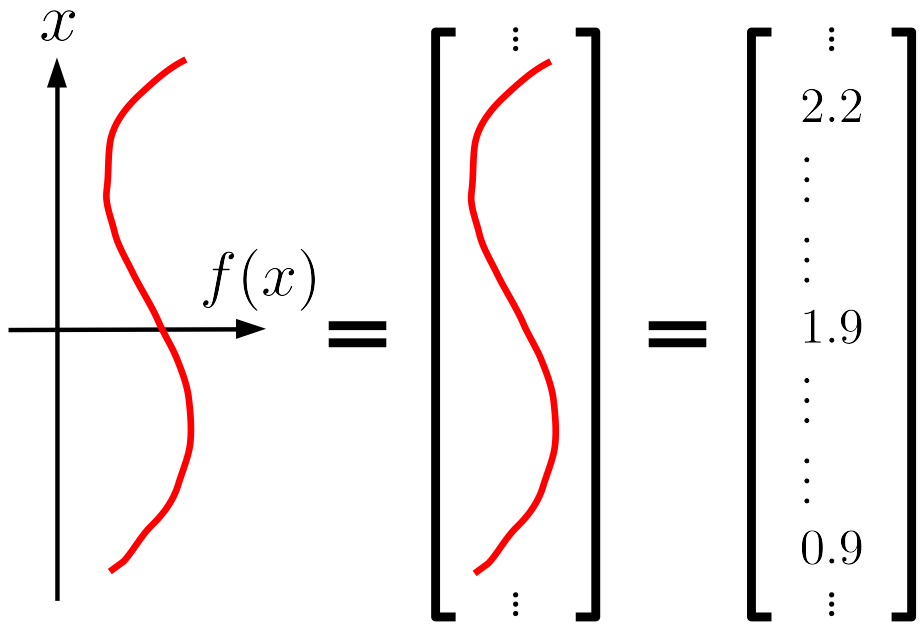
\includegraphics[width=90mm]{./figs/function_is_vector.png}
    \end{figure}
    関数のゼロベクトルを${ }^{\forall} t \ 0(t) := 0$で定める.
\end{frame}

\begin{frame}[c]
    \frametitle{関数の内積}
    2関数$f,g$の内積を次で定める:
    \begin{align}
        \innprod{f(x)}{g(x)} &:= \int_{a}^{b} f(x) \roverline{g(x)} \mathrm{d}x \label{eq:function_innerprod} \\
        \roverline{g(x)} &: \text{$g(x)$の複素共役} \nonumber
    \end{align}
    積分範囲$[a,b]$は対象により変わる.積分変数を省略して$\innprod{f}{g}$とも書く.考え方は,(可算)次元ベクトルと同じ:
    \begin{align*}
        \innprod{\ve{v}}{\ve{w}} := \sum_{n} (\ve{v})_{n} \roverline{(\ve{w})_{n}}
    \end{align*}
\end{frame}

\begin{frame}[c]
    \frametitle{関数の内積}
    内積に関する性質も有限次元ベクトルと同様
    \begin{itemize}
        \item 関数の\structure{直交性}:
            \begin{align}
                \text{関数$f$と$g$が直交} \iff \innprod{f}{g} = 0 \label{eq:function_orth}
            \end{align}
        \item 関数の\structure{ノルム}:
            \begin{align}
                \norm{f}{2}^{2} := \innprod{f}{f} \label{eq:function_norm}
            \end{align}
    \end{itemize}
\end{frame}

\begin{frame}[c]
    \frametitle{関数空間}
    関数の張るベクトル空間を\structure{関数空間}という.たとえば,ノルムが有限
    \begin{align*}
        \norm{f}{2}^{2} = \int_{-\infty}^{\infty} |f(x)|^{2} \mathrm{d}x < \infty
    \end{align*}
    な関数$f:\mathbb{R} \to \mathbb{C}$の集合は関数空間をなす.$L_{2}(\mathbb{R})$と書く.
\end{frame}

\subsection{関数空間の例:フーリエ級数}

\begin{frame}[c]
    \frametitle{関数空間の例:フーリエ級数}
    周期$T=2\pi/\omega$の関数$f$のフーリエ級数
    \begin{align}
        \left\{
            \begin{array}{l}
                \displaystyle f(t)  = \sum_{n=-\infty}^{\infty} c_{n} \exp(jn\omega t) \\
                \displaystyle c_{n} = \frac{1}{T} \int_{-T/2}^{T/2} f(t) \exp(-jn\omega t) \mathrm{d}t
            \end{array}
        \right. \label{eq:fourior_seq}
    \end{align}
    $f(t)$を$\exp(jn\omega t)$で展開していると見える.\structure{$\frac{1}{\sqrt{T}}\exp(jn\omega t)$は正規直交基底をなしている}\footnote{ここでは天下りとする.補足の補題\ref{lem:triangle_completeness}を参照}.
\end{frame}

\begin{frame}[c]
    \frametitle{関数空間の例:フーリエ級数}
    フーリエ係数$c_{n}$は$\exp$との内積の定数倍.
    \begin{align}
        c_{n} = \frac{1}{T} \innprod{f(t)}{\exp(jn\omega t)}
    \end{align}
    $n\omega$の周波数成分との類似度を測っている.
    \begin{figure}
        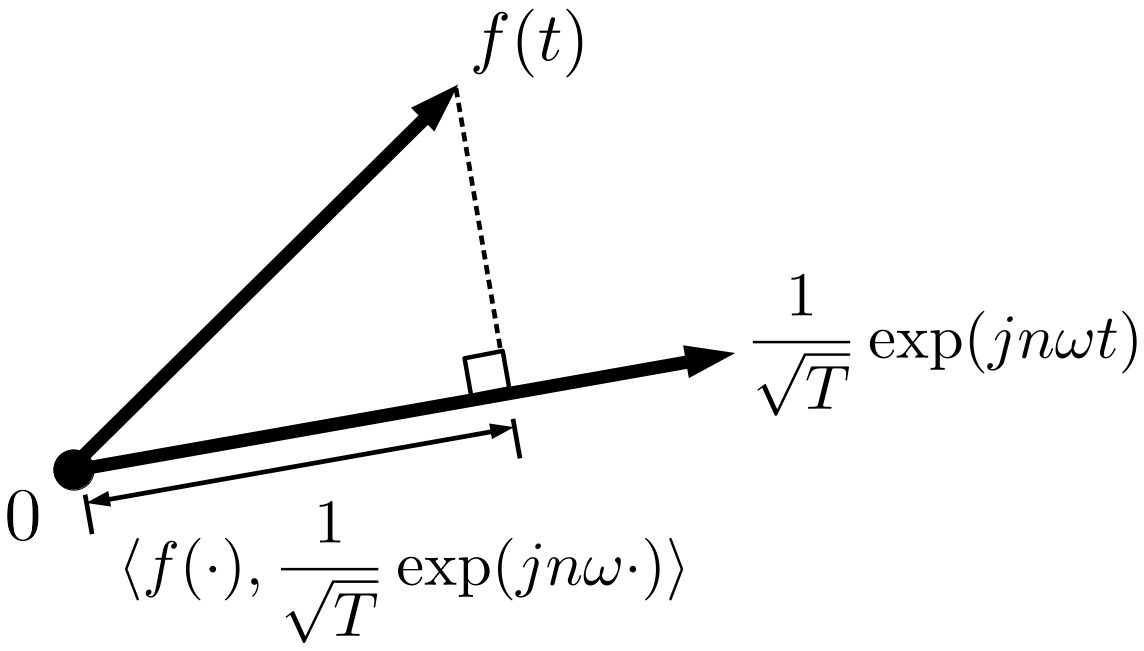
\includegraphics[width=90mm]{./figs/fourior_function_projection.png}
    \end{figure}
\end{frame}

\subsection{連続ウェーブレット変換}

\begin{frame}[c]
    \frametitle{連続ウェーブレット変換}
    空間に局在する\footnote{注意:無限範囲で値を持つものもある}"ざざ波"$\psi$を使った信号分析手法.
    \begin{itemize}
        \item $\psi$のことを\structure{ウェーブレット(Wavelet)関数}という
        \item $\psi$を時間軸方向にスケール(伸び縮み)/シフトした関数を基底とする
    \end{itemize}
\end{frame}

\begin{frame}[c]
    \frametitle{例:ハールウェーブレット$\psi_{H}$}
    \vspace*{-10pt}
    \begin{figure}
        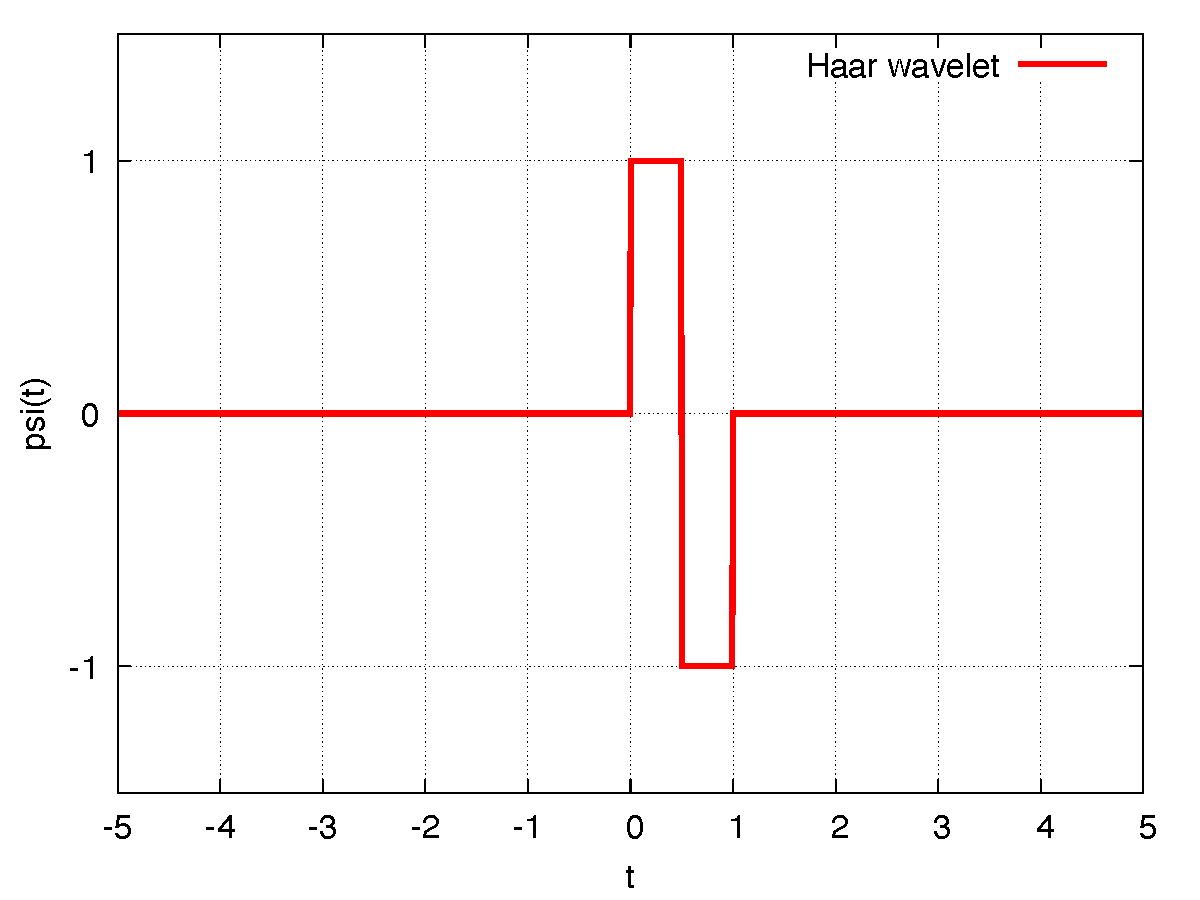
\includegraphics[width=80mm]{./figs/haar_wavelet.pdf}
    \end{figure}
    \vspace*{-5pt}
    \begin{align*}
        \psi_{H}(t) := 
        \left\{
           \begin{array}{cc}
               1  & (0 \leq t < \frac{1}{2}) \\
               -1 & (\frac{1}{2} \leq t < 1) \\
               0  & \text{otherwise}
           \end{array}
        \right. 
    \end{align*}
\end{frame}

\begin{frame}[c]
    \frametitle{例:メキシカンハットウェーブレット}
    \vspace*{-10pt}
    \begin{figure}
        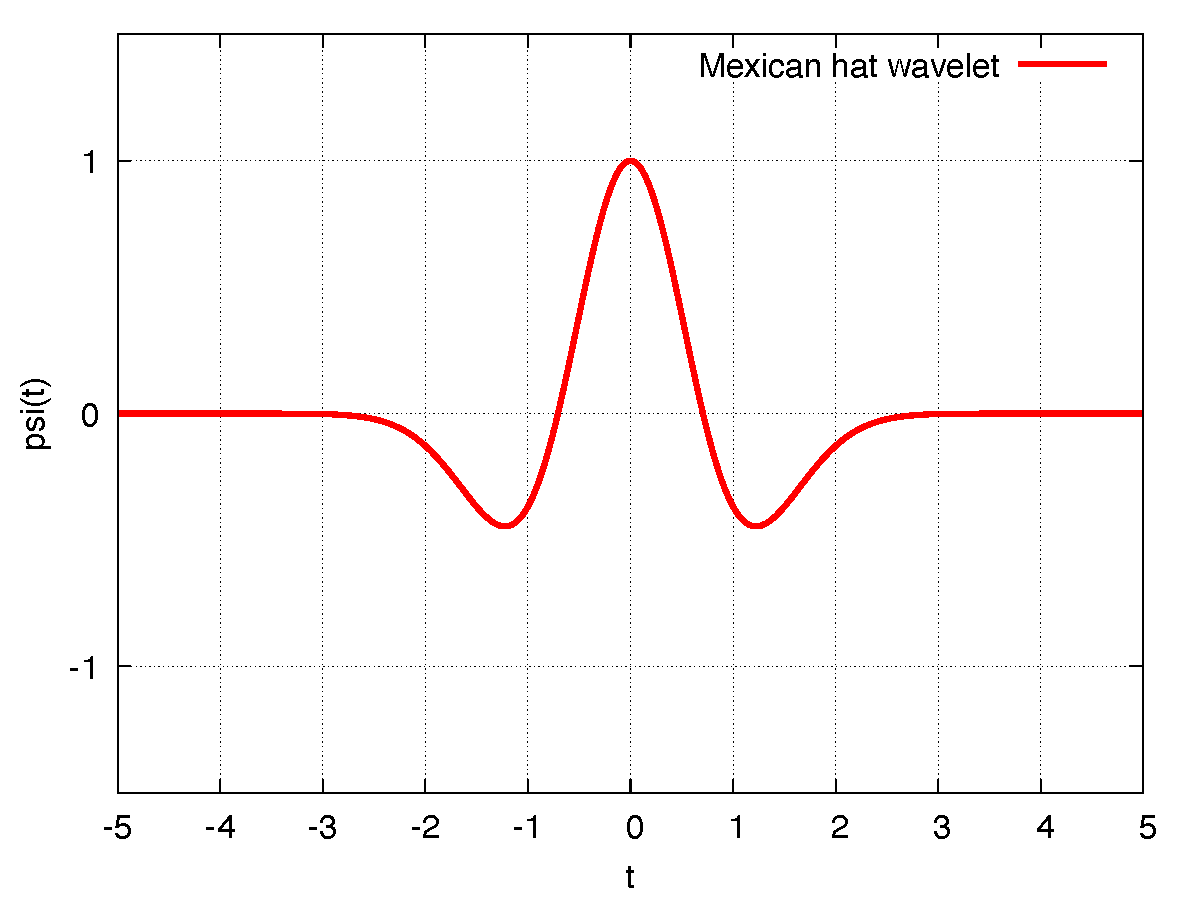
\includegraphics[width=80mm]{./figs/mexicanhat_wavelet.pdf}
    \end{figure}
    \vspace*{-5pt}
    \begin{align*}
        \psi(t) := (1 - t^{2}) \exp(-t^{2})
    \end{align*}
\end{frame}

\begin{frame}[c]
    \frametitle{例:シャノンウェーブレット}
    \vspace*{-10pt}
    \begin{figure}
        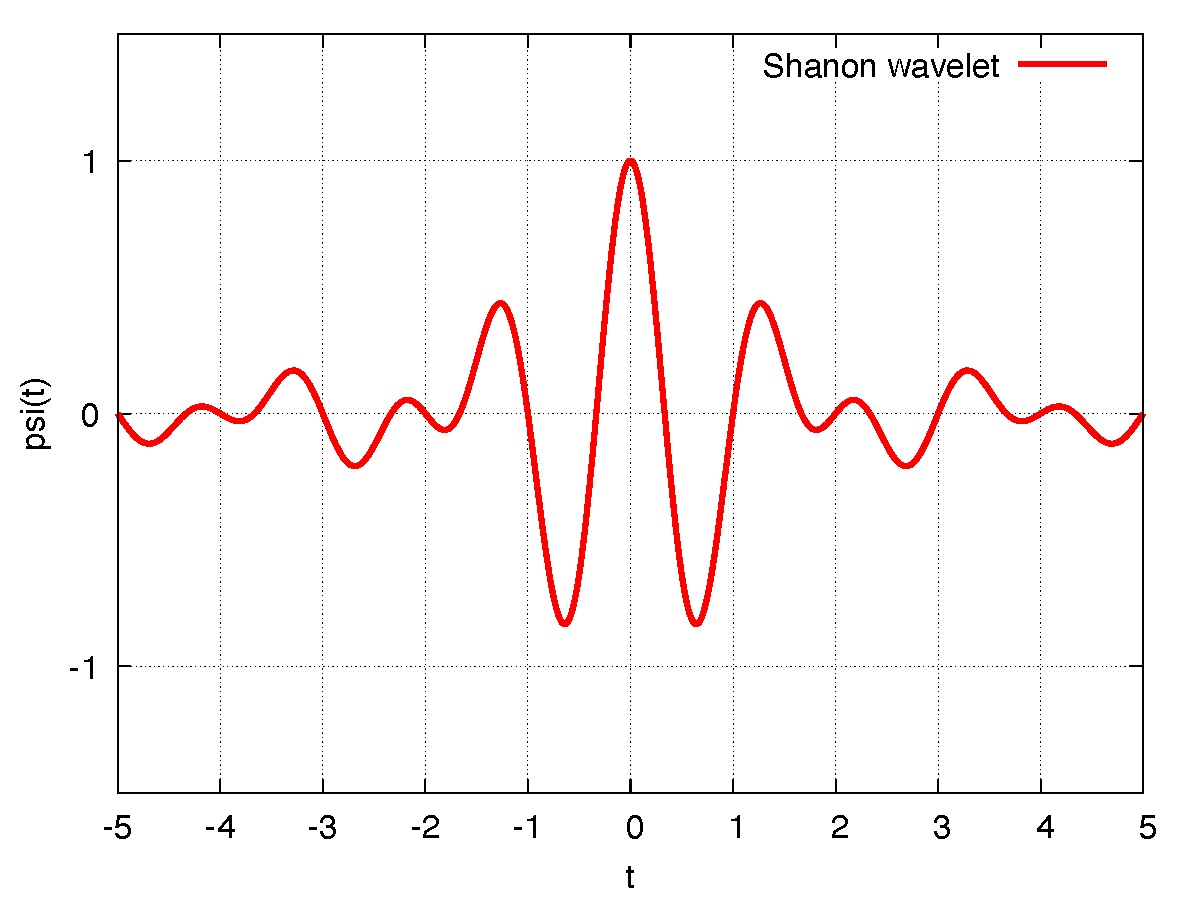
\includegraphics[width=80mm]{./figs/shanon_wavelet.pdf}
    \end{figure}
    \vspace*{-5pt}
    \begin{align*}
        \psi(t) &:= 2\mathrm{sinc}(2t) - \mathrm{sinc}(t) \\
        \mathrm{sinc}(t) &:= \frac{\sin(\pi t)}{\pi t}
    \end{align*}
\end{frame}

\begin{frame}[c]
    \frametitle{連続ウェーブレット変換}
    $\psi$に時間スケールとシフト変換を施した関数を
    \begin{align}
        \psi_{a,b}(t) := \frac{1}{\sqrt{a}} \psi\left( \frac{t - b}{a} \right) \label{eq:cont_wavelet}
    \end{align}
    と書く.$a$はスケール,$b$はシフト位置を設定.$1/\sqrt{a}$はノルムを保つための定数
    \footnote{(検算)$s = (t - b) / a$と置換積分すれば,
    \scriptsize
    \begin{align*}
        \norm{\psi_{a,b}}{2}^{2} = \int_{-\infty}^{\infty} \frac{1}{a} \psi\left( \frac{t - b}{a} \right) \roverline{\psi\left( \frac{t - b}{a} \right)} \mathrm{d}t = \frac{1}{a} \int_{-\infty}^{\infty} \psi(s) \roverline{\psi(s)} a \mathrm{d}s = \norm{\psi}{2}^{2}
    \end{align*}
    }
\end{frame}

\begin{frame}[c]
    \frametitle{例:ハールウェーブレット}
    \begin{figure}
        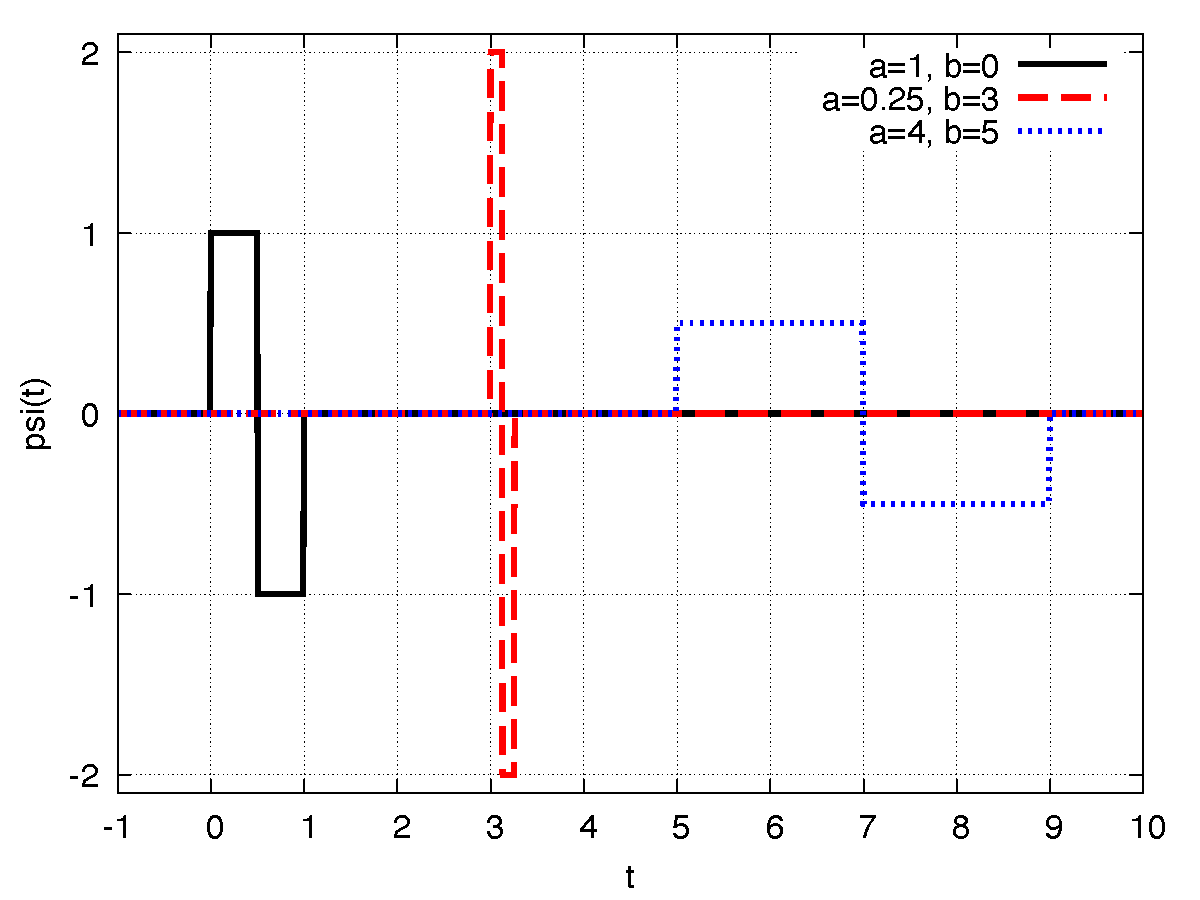
\includegraphics[width=100mm]{./figs/haar_wavelets.pdf}
    \end{figure}
\end{frame}

\begin{frame}[c]
    \frametitle{連続ウェーブレット変換}
    関数$f$の連続ウェーブレット変換$F(a,b)$は,$f$と$\psi_{a,b}$の内積によって得られる:
    \begin{align}
        F(a,b) &:= \int_{-\infty}^{\infty} f(t) \roverline{\psi_{a,b}(t)} \mathrm{d}t \\
        &= \innprod{f(t)}{\psi_{a,b}(t)} \nonumber
    \end{align}
    変換先はスケール$a$とシフト$b$の2軸(スケログラムという)
\end{frame}

\subsection{直交ウェーブレット変換}

\begin{frame}[c]
    \frametitle{ウェーブレットの離散化}
    $\psi_{a,b}$(式\eqref{eq:cont_wavelet})のスケール$a$とシフト$b$を
    \begin{align*}
        a = 2^{-m},\ b = n2^{-m}
    \end{align*}
    と整数$m,n\in \mathbb{Z}$で離散化して\footnote{文献によっては$m$の符号が逆転しているので注意!},
    \begin{align}
        \psi_{m,n}(t) &:= \frac{1}{\sqrt{2^{-m}}} \psi\left( \frac{t - n2^{-m}}{2^{-m}} \right) \nonumber \\
        &= 2^{\frac{m}{2}} \psi(2^{m}t - n)
    \end{align}
    と書く.
\end{frame}

\begin{frame}[c]
    \frametitle{直交ウェーブレット変換}
    \underline{もし},$\psi_{m,n}(t)$が正規直交基底をなす
    \begin{align*}
        {}^{\forall} i,j,k,l \in \mathbb{Z}.\ \innprod{\psi_{i,j}}{\psi_{k,l}} = \delta_{ik} \delta_{jl}
    \end{align*}
    ならば\footnote{スケール/シフトの両方で正規直交},任意の信号$x \in L_{2}(\mathbb{R})$をウェーブレット展開係数$X_{m,n} = \innprod{x}{\psi_{m,n}}$を用いて
    \begin{align}
        x(t) = \sum_{m,n} X_{m,n} \psi_{m,n}(t)
    \end{align}
    と展開できる.これを直交ウェーブレット変換という.
\end{frame}

\section{多重解像度解析(MRA)}

\subsection{多重解像度解析の概要}

\begin{frame}[c]
    \frametitle{多重解像度解析(MRA)の概要}
    \structure{多重解像度解析(MRA\footnote{MultiResolution Analysis})}は直交ウェーブレット変換の手法のひとつ.
    対象の信号を様々なスケール(解像度)に分解して解析を行う.
\end{frame}

\begin{frame}[c]
    \frametitle{多重解像度解析(MRA)の概要}
    スケール$M$の信号$f^{(M)}(t)$を1つスケールの落とした信号$f^{(M-1)}(t)$と誤差信号$g^{(M-1)}(t)$の和で表すことを考える:
    \begin{align}
        f^{(M)}(t) = f^{(M-1)}(t) + g^{(M-1)}(t) \label{eq:mra_decomp_onescale}
    \end{align}
    $M$はスケールの細かさ.大きくとればどんな信号でも近似できる.
\end{frame}

\begin{frame}[c]
    \frametitle{多重解像度解析(MRA)の概要}
    式\eqref{eq:mra_decomp_onescale}を繰り返し適用していくと,
    \begin{align}
        f^{(M)}(t) &= f^{(M-1)}(t) + g^{(M-1)}(t) \nonumber \\
        &= f^{(M-2)}(t) + g^{(M-1)}(t) + g^{(M-2)}(t) \nonumber \\
        &= ... \nonumber \\
        &= f^{(J)}(t) + \sum_{m=J}^{M-1} g^{(m)}(t) \label{eq:mra_decomp_multiscale}
    \end{align}
    任意のスケール$J < M$まで信号を分解できる!
\end{frame}

\begin{frame}[c]
    \frametitle{多重解像度解析(MRA)の概要}
    \begin{figure}
        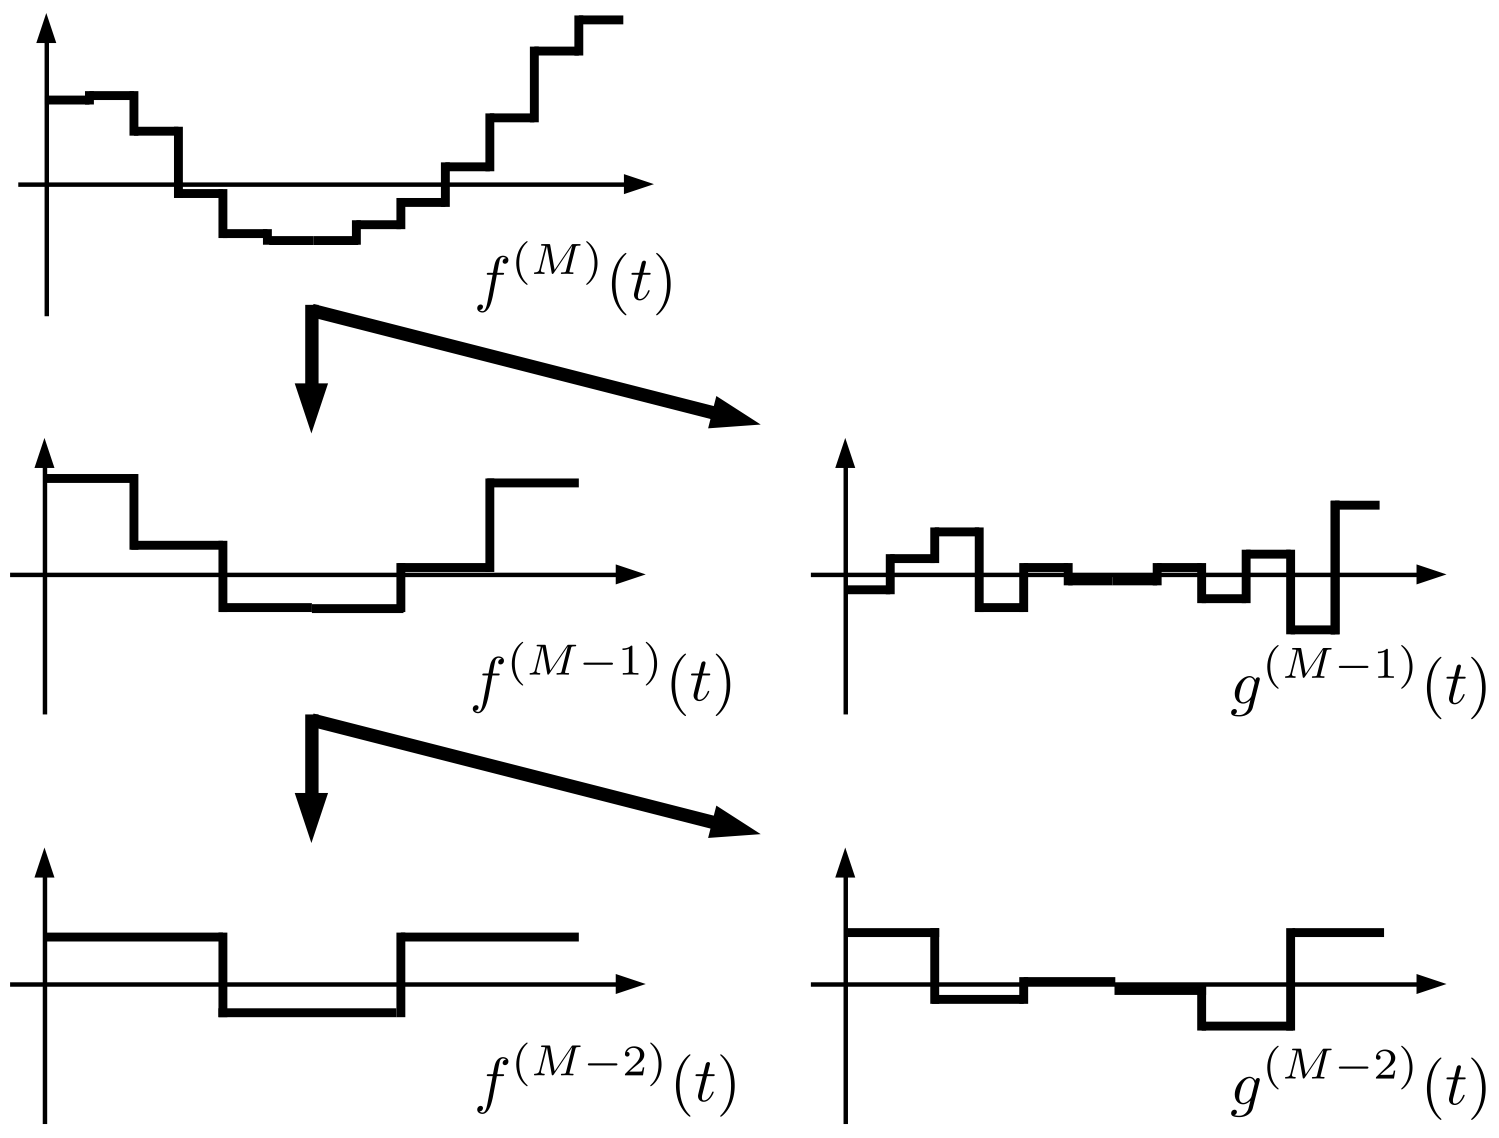
\includegraphics[width=95mm]{./figs/rma_absraction.png}
    \end{figure}
    この操作を形式的に考えていく.
\end{frame}

\subsection{多重解像度解析の条件と性質}

\begin{frame}[c]
    \frametitle{多重解像度解析(MRA)}
    MRAは次の部分空間$V_{m}$と関数$\phi$
    \begin{align}
        V_{m} &:= \left\{ \sum_{n} c_{n} \phi_{m,n}(t) \middle| c_{n} \in l_{2}(\mathbb{Z}) \right\} \\
        \phi_{m,n}(t) &:= 2^{\frac{m}{2}}\phi(2^{m}t - n)
    \end{align}
    を基に構成される\footnote{$l_{2}(\mathbb{Z})$は二乗総和可能な数列($\sum_{n} |c_{n}|^{2} < \infty$)の集合}\footnote{文献によっては$m$の符号が逆転しているので注意!}.$\phi$を\structure{スケーリング関数(scaling function)}という.
\end{frame}

\begin{frame}[c, allowframebreaks]
    \frametitle{MRAの満たすべき条件}
    MRAは,集合$V_{m}$に対して以下の条件(M1)-(M4)を要求する:
    \begin{enumerate}[(M1)]
        \item \label{itm:mra1} $V_{0}$は正規直交基底
            \begin{align*}
                \{ \phi(t - n) | n \in \mathbb{Z} \},\ \phi \in L_{2}(\mathbb{R})
            \end{align*}
            によって張られる
            \begin{itemize}
                \item[お気持ち] スケーリング関数$\phi$は整数シフトに関して正規直交基底となることを要求:
                    \begin{align*}
                        \innprod{\phi(t - n)}{\phi(t - m)} = \delta_{nm}
                    \end{align*}
            \end{itemize}
            \newpage
        \item \label{itm:mra2} $V_{m} \subset V_{m+1}$
            \begin{itemize}
                \item[お気持ち] $V_{m}$は入れ子構造をなしている.
                    \begin{figure}
                        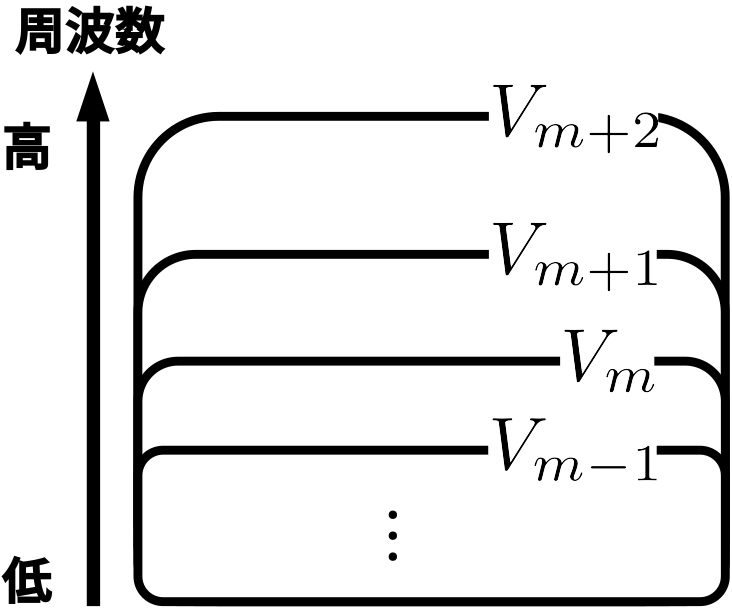
\includegraphics[width=70mm]{./figs/mra_scaling_set.png}
                    \end{figure}
                    解像度$m$を上げると表現可能な信号が増える
            \end{itemize}
            \newpage
        \item \label{itm:mra3} $\roverline{\bigcup_{m} V_{m}} = L_{2}(\mathbb{R})$($\roverline{A}$:集合$A$の閉包)
            \begin{itemize}
                \item[お気持ち] $\displaystyle\lim_{m \to \infty} V_{m} = L_{2}(\mathbb{R})$であること,つまり,$L_{2}(\mathbb{R})$のどんな信号であっても任意の精度で近似できる
            \end{itemize}
        \item $\bigcap_{m} V_{m} = \{ 0 \}$
            \begin{itemize}
                \item[お気持ち] $\displaystyle\lim_{m \to -\infty} V_{m} = \{ 0 \}$であること,つまり,解像度を極限まで落とすと$V_{m}$に含まれる信号は定値関数$0$のみになる
            \end{itemize}
    \end{enumerate}
\end{frame}

\begin{frame}[c]
    \frametitle{例:ハールウェーブレット$\psi_{H}$}
    $\psi_{H}$に対応するスケーリング関数$\phi_{H}$
    \begin{align*}
        \phi_{H}(t) := 
        \left\{
           \begin{array}{cc}
               1  & (0 \leq t < 1) \\
               0  & \text{otherwise}
           \end{array}
        \right. 
    \end{align*}
    $\phi_{H m,n}(t) := 2^{\frac{m}{2}}\phi_{H}(2^{m}t - n)$とかく.
    \vspace*{-5pt}
    \begin{figure}
        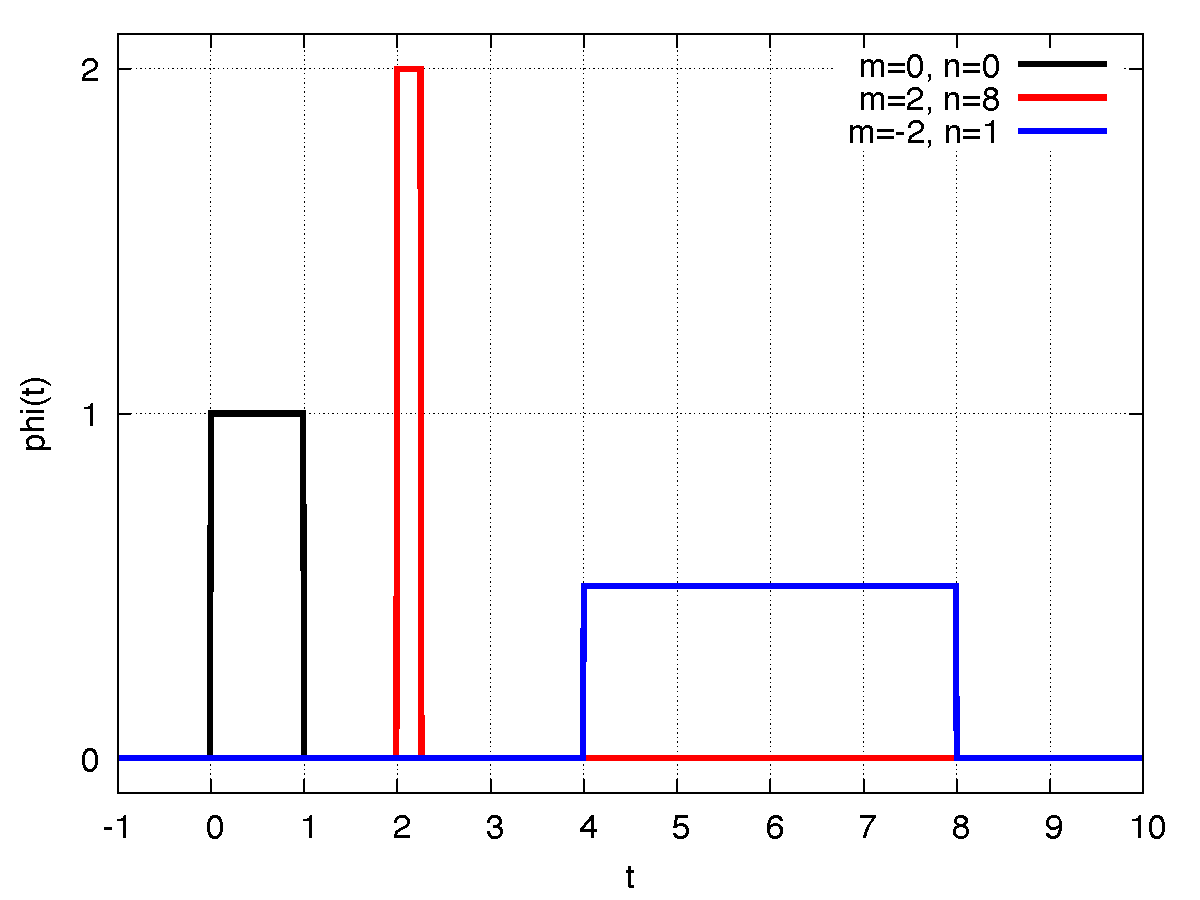
\includegraphics[width=70mm]{./figs/haar_scaling_functions.pdf}
    \end{figure}
\end{frame}

\begin{frame}[c]
    \frametitle{例:ハールウェーブレット$\psi_{H}$}
    $\phi_{H}$が条件(M\ref{itm:mra1})-(M\ref{itm:mra2})を満たすかチェック
    \begin{enumerate}[(M1)]
        \item $a,b \in \mathbb{Z}$に対して,
            \small
            \begin{align*}
                & \innprod{\phi_{H}(t-a)}{\phi_{H}(t-b)} = \int_{-\infty}^{\infty} \phi_{H}(t-a) \roverline{\phi_{H}(t-b)} \mathrm{d} t \\
                &= \int_{-\infty}^{\infty} \phi_{H}(s) \phi_{H}(s+a-b) \mathrm{d} s \quad (s = t - a) \\
                &= \delta_{ab}
            \end{align*}
            \normalsize
            なので$\{ \phi_{H}(t - n) | n \in \mathbb{Z} \}$は正規直交基底.
    \end{enumerate}
\end{frame}

\begin{frame}[c]
    \frametitle{例:ハールウェーブレット$\psi_{H}$}
    \begin{enumerate}[(M1)]
        \setcounter{enumi}{1}
        \item 任意の$m,n \in \mathbb{Z}$に対して,
            \small
            \begin{align*}
                \phi_{H m,n}(t) &= 
                \left\{
                    \begin{array}{cc}
                        2^{\frac{m}{2}} & 2^{-m}n \leq t < 2^{-m}(n+1) \\
                        0  & \text{otherwise}
                    \end{array}
                    \right. \\
                \phi_{H m+1,2n}(t) &= 
                \left\{
                    \begin{array}{cc}
                        2^{\frac{m+1}{2}} & 2^{-(m+1)} 2n \leq t < 2^{-(m+1)}(2n+1) \\
                        0  & \text{otherwise}
                    \end{array}
                    \right. \\
                    &= \left\{
                    \begin{array}{cc}
                        2^{\frac{m+1}{2}} & 2^{-m} n \leq t < 2^{-m}(n+\frac{1}{2}) \\
                        0  & \text{otherwise}
                    \end{array}
                    \right. 
            \end{align*}
            \normalsize
            だから,任意の$\phi_{H m,n} \in V_{m}$は$\phi_{H m+1,2n}, \phi_{H m+1,2n+1} \in V_{m+1}$を用いて
            \small
            \begin{align}
                \phi_{H m,n}(t) = 2^{-\frac{1}{2}} \phi_{H m+1,2n}(t) + 2^{-\frac{1}{2}} \phi_{H m+1,2n+1}(t) \label{eq:haar_dilation_eq}
            \end{align}
            \normalsize
            と表せる.よって$V_{m} \subset V_{m+1}$.
    \end{enumerate}
\end{frame}

% \begin{frame}[c]
%     \frametitle{例:ハールウェーブレット$\psi_{H}$}
%     \begin{enumerate}[(M1)]
%             \setcounter{enumi}{2}
%         \item \small
%             $\displaystyle\lim_{m\to\infty} \phi_{Hm,0}(t) = \delta(t)$($\delta(t)$:インパルス関数)の観察から,$\displaystyle\lim_{m\to\infty}V_{m}$はインパルス関数を時間シフトした集合となる.任意の$f \in L_{2}(\mathbb{R})$,$s \in \mathbb{R}$に対して$\delta(t - s) \in \displaystyle\lim_{m\to\infty}V_{m}$が存在して,
%             \begin{align*}
%                 \innprod{f(t)}{\delta(t - s)} = \int_{-\infty}^{\infty} f(t) \delta(t - s) \mathrm{d} t = f(s)
%             \end{align*}
%             だから,$f \in \displaystyle\lim_{m\to\infty}V_{m}$で$L_{2}(\mathbb{R}) \subset \displaystyle\lim_{m\to\infty}V_{m}$.一方,$\phi_{Hm,n} \in L_{2}(\mathbb{R})$だから$L_{2}(\mathbb{R})\supset \displaystyle\lim_{m\to\infty}V_{m}$.従って,$\displaystyle\lim_{m\to\infty}V_{m} = L_{2}(\mathbb{R})$.
%             \normalsize
%         \item $\displaystyle\lim_{m\to-\infty} \phi_{Hm,n}(t) = 0$より確かに$\displaystyle\lim_{m\to-\infty}V_{m}$は$0$しか含まない.
%     \end{enumerate}
% \end{frame}

\begin{frame}[c]
    \frametitle{MRAの条件から出てくる性質}
    (M\ref{itm:mra1})が成立すれば,任意の$m,p,q \in \mathbb{Z}$に対し,
    \begin{align*}
        \innprod{\phi_{m,p}}{\phi_{m,q}} &= \int_{-\infty}^{\infty} 2^{\frac{m}{2}} \phi(2^{m}t - p) \roverline{2^{\frac{m}{2}} \phi(2^{m}t - q)} \mathrm{d} t \\
        &= 2^{m} \int_{-\infty}^{\infty} \phi(2^{m}t - p) \roverline{\phi(2^{m}t - q)} \mathrm{d} t \\
        &= \int_{-\infty}^{\infty} \phi(s - p) \roverline{\phi(s - q)} \mathrm{d} s \quad (s = 2^{m}t) \\
        &= \delta_{pq} \quad \text{($\because$ $\phi$はシフトに関して正規直交)}
    \end{align*}
    だから,1つのスケーリング関数$\phi$が決まれば全ての$V_{m}$が張られる.
\end{frame}

\begin{frame}[c]
    \frametitle{Dilation方程式(ツースケール関係)}
    (M\ref{itm:mra2})が成立すれば,$V_{-1} \subset V_{0}$より,$\phi(t/2) \in V_{-1}$は$V_{0}$の基底$\{ \phi(t-n) | n \in \mathbb{Z} \}$の線形結合で表現できるから,
    \begin{align}
        \phi(t/2) = \sqrt{2} \sum_{n} h[n] \phi(t - n) \label{eq:dilation_eq}
    \end{align}
    を満たす係数$\{ h[n] \}$が存在する\footnote{$\sqrt{2}$は規格化定数}.これを\structure{Dilation方程式}とか\structure{ツースケール関係}と呼ぶ.
\end{frame}

\begin{frame}[c]
    \frametitle{MRAのウェーブレット関数}
    (M\ref{itm:mra2})より$V_{m} \subset V_{m+1}$だから,$V_{m} \oplus W_{m} = V_{m+1}$ ($\oplus$:直和)となる$W_{m}$が存在する:\\
    \begin{figure}
        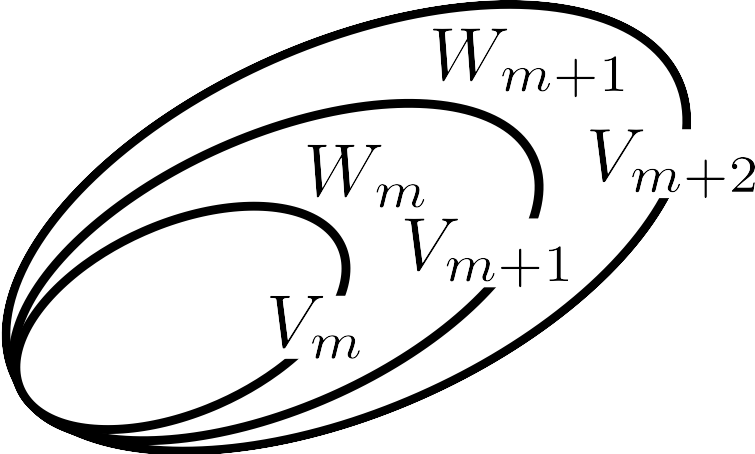
\includegraphics[width=70mm]{./figs/mra_scaling_wavelet_set.png}
    \end{figure}
\end{frame}

\begin{frame}[c]
    \frametitle{MRAのウェーブレット関数}
    $W_{m}$はスケール$m$のウェーブレットから張られるように定める:
    \begin{align}
        W_{m} := \left\{ \sum_{n} c_{n} \psi_{m,n}(t) \middle| c_{n} \in l_{2}(\mathbb{Z}) \right\}
    \end{align}
    % TODO: ここで、どのように構成すべきか指針を述べるのがいいかも。
    $V_{m} \oplus W_{m} = V_{m+1}$だから,$W_{m}$は$V_{m} \perp W_{m}$\footnote{$V_{m}, W_{m}$それぞれから選んだ任意の元が直交している}を満さなければならない.
    その成立条件を見ていこう.
\end{frame}

\begin{frame}[c]
    \frametitle{MRAのウェーブレット関数}
    $W_{-1} \subset V_{0}$だから,$\psi(t/2) \in W_{-1}$も$V_{0}$の基底$\{ \phi(t-n) | n \in \mathbb{Z} \}$の線形結合で表せて,
    \begin{align}
        \psi(t/2) = \sqrt{2} \sum_{n} g[n] \phi(t - n) \label{eq:wavelet_dilation_eq}
    \end{align}
    を満たす係数$\{ g[n] \}$が存在する.
\end{frame}

\begin{frame}[c]
    \frametitle{MRAのウェーブレット関数}
    このとき,
    \begin{block}{}
        \vspace{-17pt}
        \begin{align}
            g[n] = (-1)^{n} \roverline{h[1 - n]} \label{eq:orth_condition}
        \end{align}
    \end{block}
    とすれば$V_{m} \perp W_{m}$が満たされる\footnote{証明は長くなる.補足にて述べる(系\ref{cor:orth_condition})}.\\
    $\Rightarrow$ \structure{必要なのは$\{h[n]\}$だけ!}有名なウェーブレットは$\{h[n]\}$の数表が与えられている!
    % もうちょっと言葉を選びたい。これでMRAができるようになるので。
\end{frame}

\begin{frame}[c]
    \frametitle{例:ハールウェーブレット}
    式\eqref{eq:haar_dilation_eq}において$m=-1, n=0$とおくと,
    \begin{align*}
        \phi_{H -1,0}(t) &= 2^{-\frac{1}{2}} \phi_{H 0,0}(t) + 2^{-\frac{1}{2}} \phi_{H 0,1}(t) \\
        \iff 2^{-\frac{1}{2}} \phi_{H}(t/2) &= 2^{-\frac{1}{2}} \phi_{H}(t) + 2^{-\frac{1}{2}} \phi_{H}(t - 1) \\
        \iff \phi_{H}(t/2) &= \phi_{H}(t) + \phi_{H}(t - 1)
    \end{align*}
    Dilation方程式(式\eqref{eq:dilation_eq})と見比べると
    \begin{align*}
        h[0] = h[1] = 2^{-\frac{1}{2}}
    \end{align*}
    式\eqref{eq:orth_condition}により$g[0] = 2^{-\frac{1}{2}},\ g[1] = -2^{-\frac{1}{2}}$が得られ,
    \begin{align*}
        \psi_{H}(t/2) = \phi_{H}(t) - \phi_{H}(t - 1)
    \end{align*}
    に対応していることが確認できる.
\end{frame}

\subsection{高速ウェーブレット変換(FWT)}

\begin{frame}[c]
    \frametitle{MRAの直交ウェーブレット変換}
    $V_{m} \oplus W_{m} = V_{m+1}$を繰り返し適用すると,
    \begin{align*}
        V_{m} &= V_{m-1} \oplus W_{m-1} \\
        &= V_{m-2} \oplus W_{m-2} \oplus W_{m-1} \\
        &= ... \\
        &= V_{J} \oplus W_{J} \oplus W_{J-1} \oplus \dots \oplus W_{m-1} \quad (J < m) \\
        &= V_{J} \oplus \left( \bigoplus_{k=J}^{m-1} W_{k} \right)
    \end{align*}
    と書ける.$m\to\infty$とすると,
    \begin{align}
        \lim_{m \to \infty} V_{m} = V_{J} \oplus \left( \bigoplus_{k=J}^{\infty} W_{k} \right) \label{eq:orth_directsum_decomposition}
    \end{align}
\end{frame}

\begin{frame}[c]
    \frametitle{MRAの直交ウェーブレット変換}
    式\eqref{eq:orth_directsum_decomposition},(M\ref{itm:mra3})($\lim_{m\to\infty} V_{m} = L_{2}(\mathbb{R})$),$V_{m} \perp W_{m}\ (m \in \mathbb{Z})$より,任意の$x(t) \in L_{2}(\mathbb{R})$は以下のように直交展開できる:
    \begin{align}
        x(t) = \underbrace{\sum_{n} p_{J}[n] \phi_{J,n}(t)}_{\in V_{J}} + \sum_{m=J}^{\infty} \underbrace{\sum_{n} q_{m}[n] \psi_{m,n}(t)}_{\in W_{m}} \label{eq:orth_decomp}
    \end{align}
    ここで,$p_{m}[n] = \innprod{x}{\phi_{m,n}},\ q_{m}[n] = \innprod{x}{\psi_{m,n}}$.
\end{frame}

\begin{frame}[c]
    \frametitle{MRAの直交ウェーブレット変換}
    スケール$M > J$以上の成分を無視すると以下の近似が成り立つ:
    \begin{align}
        x(t) \approx \sum_{n} p_{J}[n] \phi_{J,n}(t) + \sum_{m=J}^{M-1}\sum_{n} q_{m}[n] \psi_{m,n}(t) \label{eq:orth_approx}
    \end{align}
    ここで,$f^{(m)}(t) := \sum_{n} p_{m} \phi_{m,n}(t)$,$g^{(m)}(t) := \sum_{n} q_{m}[n] \psi_{m,n}(t)$とすると
    \begin{align*}
        x(t) \approx f^{(J)}(t) + \sum_{m=J}^{M-1} g^{(m)}(t)
    \end{align*}
    式\eqref{eq:mra_decomp_multiscale}そのもの:多重解像度解析を構成している.
\end{frame}

\begin{frame}[c]
    \frametitle{FWTの導出(展開)}
    式\eqref{eq:orth_decomp}の展開係数$p_{m}[n], q_{m}[n]$を計算するには$\phi, \psi$が必要と思えるが,\structure{実はその必要はなく,$h[n], g[n]$を用いて計算できる}.
    \begin{mylemma}[展開係数計算]
        \vspace*{-15pt}
        \begin{align}
            p_{m}[n] &= \sum_{k} \roverline{h[k - 2n]} p_{m+1}[k] \label{eq:scaling_coef_updation} \\
            q_{m}[n] &= \sum_{k} \roverline{g[k - 2n]} p_{m+1}[k] \label{eq:wavelet_coef_updation}
        \end{align}
    \end{mylemma}
    この演算は畳み込み(FIRフィルタ)に相当
\end{frame}

\begin{frame}[c]
    \frametitle{FWTの導出(展開)}
    \scriptsize
    (証明)準備として,Dilation方程式(式\eqref{eq:dilation_eq})から導かれる関係式に着目する.
    \begin{align}
        \phi_{m,n}(t) &= 2^{\frac{m}{2}} \phi(2^{m}t - n) = 2^{\frac{m}{2}} \phi\left(\frac{2^{m+1}t - 2n}{2}\right) \nonumber \\
        &= 2^{\frac{m}{2}} \sqrt{2} \sum_{k} h[k] \phi(2^{m+1}t - 2n - k) \quad \text{($\because$ Dilation方程式)} \nonumber \\
        &= \sum_{k} h[k] 2^{\frac{m+1}{2}} \phi(2^{m+1} - 2n - k) = \sum_{k} h[k] \phi_{m+1,2n+k} (t) \label{eq:another_scale_dilation_eq}
    \end{align}
    $\psi_{m,n}$に関しても同様にして,式\eqref{eq:wavelet_dilation_eq}から,
    \begin{align}
        \psi_{m,n}(t) = \sum_{k} g[k] \phi_{m+1,2n+k} (t) \label{eq:another_wavelet_dilation_eq}
    \end{align}
    任意の$x(t) \in L_{2}(\mathbb{R})$をとる.式\eqref{eq:another_scale_dilation_eq},式\eqref{eq:another_wavelet_dilation_eq}を用いると,
    \begin{align*}
        p_{m}[n] &= \innprod{x}{\phi_{m,n}} = \innprod{x}{\sum_{k} h[k] \phi_{m+1,2n+k}} = \sum_{k} \roverline{h[k]} \innprod{x}{\phi_{m+1,2n+k}} \\
        &= \sum_{k} \roverline{h[k]} p_{m+1}[2n+k] = \sum_{k} \roverline{h[k - 2n]} p_{m+1}[k] \quad (k \leftarrow 2n + k) \\
        q_{m}[n] &= \innprod{x}{\psi_{m,n}} = \innprod{x}{\sum_{k} g[k] \phi_{m+1,2n+k}} = \sum_{k} \roverline{g[k - 2n]} p_{m+1}[k]
    \end{align*}
\end{frame}

\begin{frame}[c]
    \frametitle{FWTの導出(再構成)}
    逆に,\structure{$h[n], g[n]$を用いて$p_{m}[n], q_{m}[n]$から$p_{m+1}[n]$を再構成できる}.
    \begin{mylemma}[再構成計算]
        \vspace*{-15pt}
        \begin{align}
            p_{m+1}[n] = \sum_{k} h[n-2k] p_{m}[k] + \sum_{k} g[n-2k] q_{m}[k] \label{eq:scaling_coef_reconstraction} 
        \end{align}
    \end{mylemma}
    式\eqref{eq:scaling_coef_updation},式\eqref{eq:wavelet_coef_updation},式\eqref{eq:scaling_coef_reconstraction}による逐次的な展開・再構成アルゴリズムを\structure{高速ウェーブレット変換(FWT, Fast Wavelet Transform)}という.
\end{frame}

\begin{frame}[c]
    \frametitle{FWTの導出(再構成)}
    \scriptsize
    (証明)$p_{m+1}[n]$の定義と$x$の直交展開式(式\eqref{eq:orth_decomp})より,
    \begin{align*}
        p_{m+1}[n] &= \innprod{x}{\phi_{m+1}[n]} \\
        &= \innprod{\sum_{k} p_{m}[k] \phi_{m,k} + \sum_{t=m}^{\infty}\sum_{k} q_{t}[k] \psi_{t,k}}{\phi_{m+1,n}} \\
        &= \sum_{k} p_{m}[k] \innprod{\phi_{m,k}}{\phi_{m+1,n}} + \sum_{t=m}^{\infty} \sum_{k} q_{t}[k] \innprod{\psi_{t,k}}{\phi_{m+1,n}}
    \end{align*}
    ここで,式\eqref{eq:another_scale_dilation_eq}より,
    \begin{align*}
        \innprod{\phi_{m,k}}{\phi_{m+1,n}} &= \innprod{\sum_{l} h[l] \phi_{m+1,2k+l}}{\phi_{m+1,n}} \\
        &= \innprod{\sum_{s} h[s-2k] \phi_{m+1,s}}{\phi_{m+1,n}} \quad (s = 2k + l) \\
        &= \sum_{s} h[s-2k] \innprod{\phi_{m+1,s}}{\phi_{m+1,n}} \\
        &= \sum_{s} h[s-2k] \delta_{sn} \quad \text{($\because$ $\phi$のシフトに関する直交性)} \\
        &= h[n-2k]
    \end{align*}
\end{frame}

\begin{frame}[c]
    \frametitle{FWTの導出(再構成)}
    \scriptsize
    任意の$t \geq m+1$に対して(M\ref{itm:mra2})より$V_{m+1} \subset V_{t}$だから,
    \begin{align*}
        W_{t} \perp V_{t} \implies W_{t} \perp V_{m+1}
    \end{align*}
    よって$\innprod{\psi_{t, k}}{\phi_{m+1,n}} = 0\ (t \geq m+1)$.これより,
    \begin{align*}
        \sum_{t=m}^{\infty} &\innprod{\psi_{t,k}}{\phi_{m+1,n}} = \innprod{\psi_{m,k}}{\phi_{m+1,n}} \\
        &= \innprod{\sum_{l} g[l] \phi_{m+1,2k+l}}{\phi_{m+1,n}} \quad \text{($\because$ 式\eqref{eq:another_wavelet_dilation_eq})} \\
        &= \innprod{\sum_{s} g[s-2k] \phi_{m+1,s}}{\phi_{m+1,n}} \quad (s = 2k + l) \\
        &= \sum_{s} g[s-2k] \innprod{\phi_{m+1,s}}{\phi_{m+1,n}} = \sum_{s} g[s-2k] \delta_{sn} \quad \text{($\because$ $\phi$のシフトに関する直交性)} \\
        &= g[n-2k]
    \end{align*}
    以上の結果から,
    \begin{align*}
        p_{m+1}[n] &= \sum_{k} p_{m}[k] \innprod{\phi_{m,k}}{\phi_{m+1,n}} + \sum_{t=m}^{\infty} \sum_{k} q_{t}[k] \innprod{\psi_{t,k}}{\phi_{m+1,n}} \\
        &= \sum_{k} h[n-2k] p_{m}[k] + \sum_{k} g[n-2k] q_{m}[k]
    \end{align*}
\end{frame}

\begin{frame}[c]
    \frametitle{FWTのフィルタ表現}
    展開処理(式\eqref{eq:scaling_coef_updation},\eqref{eq:wavelet_coef_updation})をフィルタ表現すると
    \begin{figure}
        \centering
        \begin{tikzpicture}[auto, >=latex']
            \renewcommand{\dspfilterwidth}{10mm}
            \newcommand{\dspfilterheight}{5mm}
            \tikzset{dspfilter/.append style = {minimum height=\dspfilterheight}}
            \newcommand{\dspvspace}{5mm}

            % Blocks and nodes
            \node(input) {};

            \node[dspfilter, right=of input, right=3.0*\dspvspace, fill=white] (Hm1) {$\roverline{H}$};
            \node[dspnodefull] (Pm1node) at ($(input)!0.5!(Hm1)$) {};
            \node[dspfilter, below=of Pm1node, below=1.0*\dspvspace, fill=white] (Gm1) {$\roverline{G}$};
            \node[dspfilter, below=of Gm1, below=0.6*\dspvspace, fill=white] (GDm1) {$\downarrow 2$};
            \node[below=of GDm1, below=1.0*\dspvspace, fill=white] (Qm) {\small $q_{m}$};
            \node[dspfilter, right=of Hm1, right=0.6*\dspvspace, fill=white] (HDm1) {$\downarrow 2$};

            \node[dspfilter, right=of HDm1, right=3.0*\dspvspace, fill=white] (Hm) {$\roverline{H}$};
            \node[dspnodefull] (Pmnode) at ($(HDm1)!0.5!(Hm)$) {};
            \node[dspfilter, below=of Pmnode, below=1.0*\dspvspace, fill=white] (Gm) {$\roverline{G}$};
            \node[dspfilter, below=of Gm, below=0.6*\dspvspace, fill=white] (GDm) {$\downarrow 2$};
            \node[below=of GDm, below=1.0*\dspvspace, fill=white] (Qm_1) {\small $q_{m-1}$};
            \node[dspfilter, right=of Hm, right=0.6*\dspvspace, fill=white] (HDm) {$\downarrow 2$};

            % \node[dspfilter, right=of HDm, right=3.0*\dspvspace, fill=white] (Hm_1) {$\roverline{H}$};
            \node[right=of HDm, right=3.0*\dspvspace, fill=white] (Hm_1) {};
            \node[dspnodefull] (Pm_1node) at ($(HDm)!0.5!(Hm_1)$) {};
            \node[dspfilter, below=of Pm_1node, below=1.0*\dspvspace, fill=white] (Gm_1) {$\roverline{G}$};
            \node[dspfilter, below=of Gm_1, below=0.6*\dspvspace, fill=white] (GDm_1) {$\downarrow 2$};
            \node[below=of GDm_1, below=1.0*\dspvspace, fill=white] (Qm_2) {\small $q_{m-2}$};
            % \node[dspfilter, right=of Hm, right=0.6*\dspvspace, fill=white] (HDm_1) {$\downarrow 2$};

            % Connections
            \draw[dspconn] (input) -- node[above] {\small $p_{m+1}$} (Hm1);
            \draw[dspconn] (Pm1node) -- (Gm1);
            \draw[dspconn] (Gm1) -- (GDm1);
            \draw[dspconn] (GDm1) -- (Qm);
            \draw[dspconn] (Hm1) -- (HDm1);

            \draw[dspconn] (HDm1) -- node[above] {\small $p_{m}$} (Hm);
            \draw[dspconn] (Pmnode) -- (Gm);
            \draw[dspconn] (Gm) -- (GDm);
            \draw[dspconn] (GDm) -- (Qm_1);
            \draw[dspconn] (Hm) -- (HDm);

            \draw[dspconn] (HDm) -- node[above] {\small $p_{m-1}$} (Hm_1);
            \draw[dspconn] (Pm_1node) -- (Gm_1);
            \draw[dspconn] (Gm_1) -- (GDm_1);
            \draw[dspconn] (GDm_1) -- (Qm_2);
            % \draw[dspconn] (Hm_1) -- (HDm);
        \end{tikzpicture}
        \caption{展開処理} \label{fig:decomposition_procedure}
    \end{figure}
    \structure{$\roverline{H}$はローパスフィルタ,$\roverline{G}$はハイパスフィルタ}
    \begin{itemize}
        \item $p_{m}$はスケールを落とした信号成分,$q_{m}$は差分成分だから
    \end{itemize}
\end{frame}

\begin{frame}[c]
    \frametitle{FWTのフィルタ表現}
    再構成処理(式\eqref{eq:scaling_coef_reconstraction})をフィルタ表現すると
    \begin{figure}
        \centering
        \begin{tikzpicture}[auto, >=latex']
            \renewcommand{\dspfilterwidth}{10mm}
            \newcommand{\dspfilterheight}{5mm}
            \tikzset{dspfilter/.append style = {minimum height=\dspfilterheight}}
            \newcommand{\dspvspace}{5mm}

            % Blocks and nodes
            \node(input) {};

            \node[dspfilter, right=of input, right=2.0*\dspvspace, fill=white] (HIm_1) {$\uparrow 2$};
            \node[dspfilter, right=of HIm_1, right=0.6*\dspvspace, fill=white] (Hm_1) {$H$};
            \node[dspadder, right=of Hm_1, right=1.0*\dspvspace, fill=white] (Pmadd) {};
            \node[dspfilter, below=of Pmadd, below=1.0*\dspvspace, fill=white] (Gm_1) {$G$};
            \node[dspfilter, below=of Gm_1, below=0.6*\dspvspace, fill=white] (GIm_1) {$\uparrow 2$};
            \node[below=of GIm_1, below=1.0*\dspvspace, fill=white] (Qm_1) {\small $q_{m-1}$};

            \node[dspfilter, right=of Pmadd, right=2.0*\dspvspace, fill=white] (HIm) {$\uparrow 2$};
            \node[dspfilter, right=of HIm, right=0.6*\dspvspace, fill=white] (Hm) {$H$};
            \node[dspadder, right=of Hm, right=1.0*\dspvspace, fill=white] (Pm1add) {};
            \node[dspfilter, below=of Pm1add, below=1.0*\dspvspace, fill=white] (Gm) {$G$};
            \node[dspfilter, below=of Gm, below=0.6*\dspvspace, fill=white] (GIm) {$\uparrow 2$};
            \node[below=of GIm, below=1.0*\dspvspace, fill=white] (Qm) {\small $q_{m}$};

            \node[right=of Pm1add, right=2.0*\dspvspace, fill=white] (HIm1) {};

            % Connections
            \draw[dspconn] (input) -- node[above] {\small $p_{m-1}$} (HIm_1);
            \draw[dspconn] (HIm_1) -- (Hm_1);
            \draw[dspconn] (Hm_1) -- (Pmadd);
            \draw[dspconn] (Gm_1) -- (Pmadd);
            \draw[dspconn] (GIm_1) -- (Gm_1);
            \draw[dspconn] (Qm_1) -- (GIm_1);

            \draw[dspconn] (Pmadd) -- node[above] {\small $p_{m}$} (HIm);
            \draw[dspconn] (HIm) -- (Hm);
            \draw[dspconn] (Hm) -- (Pm1add);
            \draw[dspconn] (Gm) -- (Pm1add);
            \draw[dspconn] (GIm) -- (Gm);
            \draw[dspconn] (Qm) -- (GIm);

            \draw[dspconn] (Pm1add) -- node[above] {\small $p_{m+1}$} (HIm1);

        \end{tikzpicture}
        \caption{再構成処理} \label{fig:composition_procedure}
    \end{figure}
\end{frame}

\begin{frame}[c]
    \frametitle{FWTの計算量}
    \begin{block}{}
        FWTの時間的計算量は,入力データ個数$N$に対して$\mathcal{O}(N)$.
    \end{block}
    \scriptsize
    (証明)$p_{M}[n]$が$N$個のデータからなり,$H, G$を長さ$L$のFIRフィルタとすると,各解像度における積和演算回数は次のようになる:
    \begin{itemize}
        \item[1段目] $p_{M-1}[n]$は$N/2$個のデータからなるため,$p_{M-1}[n]$の計算で$NL/2$回の積和演算,$q_{M-1}[n]$の計算で$NL/2$回の積和演算 $\Rightarrow$ 計$NL$回
        \item[2段目] $p_{M-2}[n]$は$N/4$個のデータからなるため,$p_{M-2}[n]$の計算で$NL/4$回の積和演算,$q_{M-2}[n]$の計算で$NL/4$回の積和演算 $\Rightarrow$ 計$NL/2$回
        \item[3段目] $p_{M-3}[n]$は$N/8$個のデータからなるため,$p_{M-3}[n]$の計算で$NL/8$回の積和演算,$q_{M-3}[n]$の計算で$NL/8$回の積和演算 $\Rightarrow$ 計$NL/4$回
        \item[] ...
    \end{itemize}
    よってすべての段の積和演算回数の和は,
    \begin{align*}
        NL + \frac{NL}{2} + \frac{NL}{4} + ... \leq 2NL
    \end{align*}
    再構成処理においても逆向きの手順の計算を行うだけなので計算量は変わらない.従って,計算量は$\mathcal{O}(N)$.
\end{frame}

\begin{frame}[c]
    \frametitle{展開係数の入力による近似}
    \begin{mylemma}[係数の近似\cite{boggess2015}]
        $M$は十分に大きいとする.$x$が連続かつ$\phi$がコンパクトサポート\footnote{有界な範囲外では常に$0$となっていること}ならば,
        \begin{align}
            \begin{aligned}
                p_{M}[n] &\approx A x(2^{-M}n) \\
                A &= \int_{-\infty}^{\infty} \roverline{\phi(t)} \mathrm{d} t
            \end{aligned}
        \end{align}
    \end{mylemma}
    $\Rightarrow$ 入力信号系列をそのまま分解・再構成に突っ込んで(ほぼ)OK!\footnote{ハールウェーブレットなら$A=1$}
\end{frame}

\begin{frame}[c]
    \frametitle{展開係数の入力による近似}
    \scriptsize
    (証明)$\phi$は仮定より,ある範囲$[-L,L]$だけで非ゼロ値を持つ.このとき$p_{M}[n]$は,
    \begin{align*}
        p_{M}[n] &= \innprod{x}{\phi_{M,n}} = \int_{-\infty}^{\infty} x(s) \roverline{\phi_{M,n}(s)} \mathrm{d} s = \int_{-\infty}^{\infty} x(s) \roverline{2^{M}\phi(2^{M}s - n)} \mathrm{d} s \\
        &= \int_{-\infty}^{\infty} x(2^{-M}t + 2^{-M}n) \roverline{2^{M}\phi(t)} 2^{-M} \mathrm{d} t \quad (t = 2^{M}s - n) \\
        &= \int_{-\infty}^{\infty} x(2^{-M}t + 2^{-M}n) \roverline{\phi(t)} \mathrm{d} t \\
        &= \int_{-L}^{L} x(2^{-M}t + 2^{-M}n) \roverline{\phi(t)} \mathrm{d} t \quad \text{($\because$ $\phi$はコンパクトサポート)}
    \end{align*}
    $M$が十分大きいとき,$x$の連続性により区間$[-2^{-M}L + 2^{-M}n, 2^{-M}L + 2^{-M}n]$で$x$はほぼ一定とみなせるから(図!!),
    \begin{align*}
        x(2^{-M}t + 2^{-M}n) \approx x(2^{-M}n)
    \end{align*}
    この近似により,
    \begin{align*}
        p_{M}[n] &\approx \int_{-L}^{L} x(2^{-M}n) \roverline{\phi(t)} \mathrm{d} t = x(2^{-M}n) \int_{-L}^{L} \roverline{\phi(t)} \mathrm{d} t \\
        &= x(2^{-M}n) \int_{-\infty}^{\infty} \roverline{\phi(t)} \mathrm{d} t \quad \text{($\because$ $\phi$はコンパクトサポート)} \\
        &= A x(2^{-M}n)
    \end{align*}
\end{frame}

\begin{frame}[c]
    \frametitle{FWTの特徴}
    特徴
    \begin{itemize}
        \item 式\eqref{eq:orth_condition}($g[n] := (-1)^{n}\roverline{h[1 - n]}$)より実行に必要なのは$h[n]$のみ!!
            \begin{itemize}
                \item 有名なウェーブレットは$h[n]$が公開されている
            \end{itemize}
        \item 計算量は$\mathcal{O}(N)$!!
        \item 実用上は入力信号をそのまま使用できる!!
    \end{itemize}
    注意点
    \begin{itemize}
        \item スケールは$2$の指数に限る(FFTは等間隔スケール)
        \item 不確定性原理(補足参照)を超越したわけではない
    \end{itemize}
\end{frame}

\section{実装}

\subsection{Pythonによる実装}

\subsubsection{1次元FWT}

\begin{frame}[c]
    \frametitle{ウェーブレット係数の計算(\texttt{fwt.py})}
    \lstinputlisting[language={Python}, linerange={28-33,99999-999999}, firstnumber=28, label=fwt1d]{../implementation/fwt.py}
    \small
    フィルタ係数条件(式\eqref{eq:orth_condition})において,
    \begin{align*}
        g[n] = (-1)^{n} \roverline{h[1 - n]} = (-1)^{n} \roverline{h[L + 1 - n]}
    \end{align*}
    だから($L$:フィルタ係数長.離散フーリエ変換の性質より周期性を持つ),$n$の範囲を$0,...,L-1$に直すと,
    \begin{align*}
        g[n] = (-1)^{n} \roverline{h[L - 1 - n]} \quad (n = 0, ..., L-1)
    \end{align*}
\end{frame}

\begin{frame}[c]
    \frametitle{FWTの実装例(\texttt{fwt.py})}
    \lstinputlisting[language={Python}, linerange={36-49,99999-999999}, firstnumber=36, label=fwt1d]{../implementation/fwt.py}
\end{frame}

\begin{frame}[c]
    \frametitle{IFWTの実装例(\texttt{fwt.py})}
    \lstinputlisting[language={Python}, linerange={52-68,99999-999999}, firstnumber=52, label=ifwt1d]{../implementation/fwt.py}
\end{frame}

\subsubsection{2次元FWT}

\begin{frame}[c]
    \frametitle{2次元FWTの考え方}
    縦/横方向にFWTを適用すればOK.
    \begin{figure}
        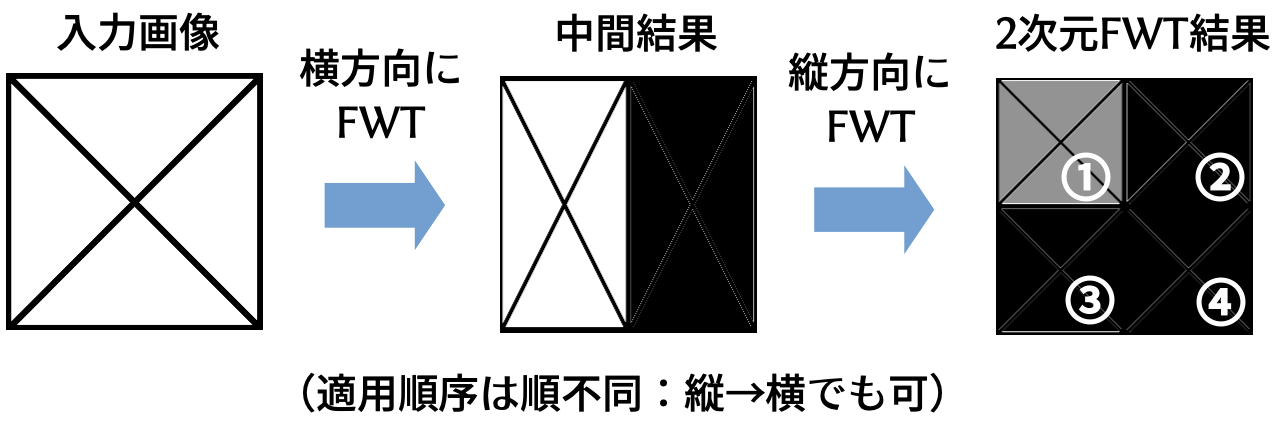
\includegraphics[width=90mm]{./figs/2dfwt_description.png}
        \caption{結果を横/縦の成分で示すと,\circled{1}=低域/低域,\circled{2}=高域/低域,\circled{3}=低域/高域,\circled{4}=高域/高域}
    \end{figure}
\end{frame}

\begin{frame}[c]
    \frametitle{2次元FWTの実装例(\texttt{fwt.py})}
    \lstinputlisting[language={Python}, linerange={71-72,99999-999999}, firstnumber=71, label=fwt2d]{../implementation/fwt.py}
    \lstinputlisting[language={Python}, linerange={81-94,99999-999999}, firstnumber=81, label=fwt2d]{../implementation/fwt.py}
\end{frame}

\begin{frame}[c]
    \frametitle{2次元IFWTの実装例(\texttt{fwt.py})}
    \lstinputlisting[language={Python}, linerange={97-111,99999-999999}, firstnumber=97, label=ifwt2d]{../implementation/fwt.py}
\end{frame}

\subsection{静止画への適用}

\begin{frame}[c]
    \frametitle{静止画の分解}
    低域/低域の結果に繰り返し2次元FWTを適用することでピラミッドを構築できる.
    \begin{figure}
        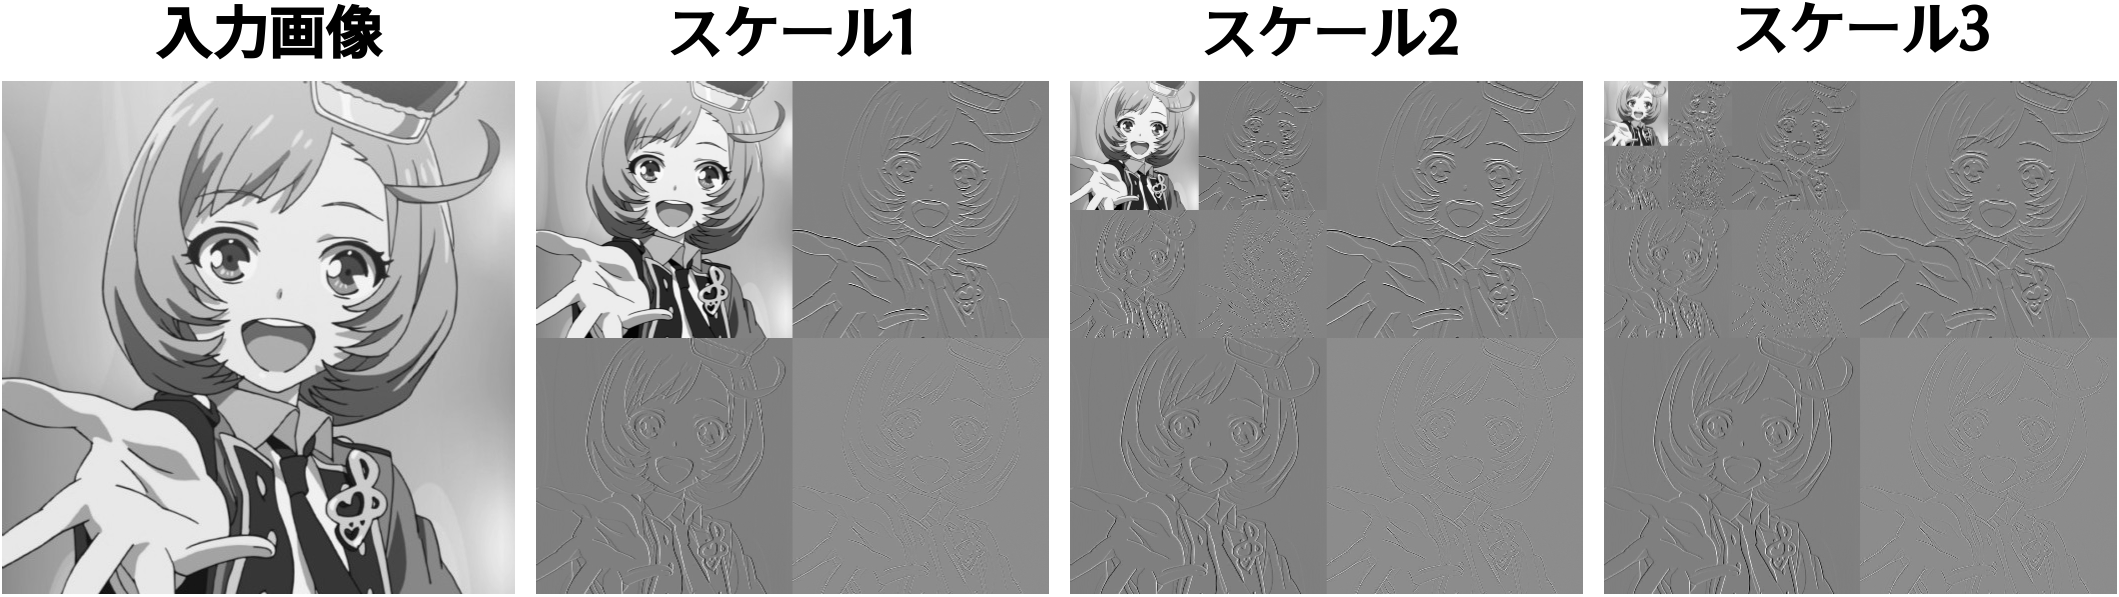
\includegraphics[width=115mm]{./figs/naru_mra_decomp.png}
    \end{figure}
\end{frame}

\begin{frame}[c]
    \frametitle{他の応用}
    NoteBook参照.以下のコンテンツを予定.
    \begin{itemize}
        \item 分解・再構成
        \item ノイズ除去
        \item 圧縮
    \end{itemize}
\end{frame}

\appendix
\setcounter{section}{0}
\renewcommand\insertsectionnumber{\Alph{section}}

\section{三角関数の完全性}

\begin{frame}[c]
    \frametitle{素朴な疑問}
    周期$T$の関数$f(x)$が以下のようにフーリエ級数展開できるとしよう.
    \begin{align*}
        f(x) &= \sum_{n} c_{n} \exp(jn\omega x) \\
        c_{n} &= \frac{1}{T} \int_{-\frac{T}{2}}^{\frac{T}{2}} f(x) \exp(-jn\omega x) \mathrm{d} x
    \end{align*}
    いや待てよ:
    \begin{itemize}
        \item 三角関数の和で$f$って表現できるの?
        \item できたとして,$f$にはどんな条件が必要?
    \end{itemize}
\end{frame}

\subsection{ディリクレ核}

\begin{frame}[c]
    \frametitle{ディリクレ核}
    一旦フーリエ級数展開ができると受け入れて,フーリエ級数の式から$c_{n}$を消して整理してみる:
    \footnotesize
    \begin{align*}
        f(x) &= \sum_{n} c_{n} \exp(jn\omega x) \\
         &= \sum_{n} \left\{ \frac{1}{T} \int_{-\frac{T}{2}}^{\frac{T}{2}} f(s) \exp(-jn\omega s) \mathrm{d} s \right\} \exp(jn\omega x) \\
         &= \frac{1}{T} \int_{-\frac{T}{2}}^{\frac{T}{2}} f(s) \sum_{n} \exp[-jn\omega(x-s)] \mathrm{d} s \\
         &= \frac{1}{T} \int_{x-\frac{T}{2}}^{x+\frac{T}{2}} f(x-u) \sum_{n} \exp(jn\omega u) \mathrm{d} u  \quad (u = x - s) \\
         &= \frac{1}{T} \int_{-\frac{T}{2}}^{\frac{T}{2}} f(x-u) \sum_{n} \exp(jn\omega u) \mathrm{d} u \quad \text{($\because$ $f$は周期$T$)}
    \end{align*}
\end{frame}

\begin{frame}[c]
    \frametitle{ディリクレ核}
    ここで,以下のディリクレ核(Dirichlet Kernel)$D_{N}$を定義する:
    \begin{align}
        D_{N}(x) = \sum_{n=-N}^{N} \exp(jnx)
    \end{align}
    $f$は$D_{N}$との畳込みで復元できる:
    \begin{align*}
        f(x) = \frac{1}{T} \int_{-\frac{T}{2}}^{\frac{T}{2}} f(x-u) D_{\infty}(\omega u) \mathrm{d} u
    \end{align*}
    $D_{N}$の性質を観察してみよう
\end{frame}

\begin{frame}[c]
    \frametitle{ディリクレ核}
    \begin{block}{}
        $D_{N}$は和を使わない式でも表現できる:
        \begin{align}
            D_{N}(x) = \frac{\sin\left\{\left(\frac{1}{2} + N\right)x\right\}}{\sin\left(\frac{1}{2}x\right)} \label{eq:dirichlet_kernel_sin}
        \end{align}
    \end{block}
    \scriptsize
    (証明)まず,
    \begin{align}
        D_{N}(x) &= \sum_{n=-N}^{N} \exp(jnx) \nonumber \\
        &= \exp(0) + \sum_{n=1}^{N} \left\{ \exp(jnx) + \exp(-jnx) \right\} \nonumber \\
        &= 1 + \sum_{n = 1}^{N} \left\{ \cos(nx) + j\sin(nx) + \cos(nx) - j\sin(nx)\right\} \nonumber \\
        &= 1 + 2 \sum_{n = 1}^{N} \cos(nx) \label{eq:dirichlet_kernel_cos}
    \end{align}
    より,$D_{N}$は$\cos$の和で表現できる.
\end{frame}

\begin{frame}[c]
    \frametitle{ディリクレ核}
    \scriptsize
    両辺$\sin\left(\frac{1}{2}x\right)$を乗じると,
    \begin{align*}
        & \sin\left(\frac{1}{2}x\right) D_{N}(x) = 2\sin\left(\frac{1}{2}x\right) \left\{ 1 + 2 \sum_{n = 1}^{N} \cos(nx) \right\} \\
        &= \sin\left(\frac{1}{2}x\right) + 2 \sin\left(\frac{1}{2}x\right)\left\{ \cos(x) + \cos(2x) + \cos(3x) + ... + \cos(Nx) \right\} \\
        &= \sin\left(\frac{1}{2}x\right) + \left[ \sin \left(\frac{1}{2} - 1\right)x + \sin \left(\frac{1}{2} + 1\right)x \right] \\
        &\quad + \left[ \sin \left(\frac{1}{2} - 2\right)x + \sin \left(\frac{1}{2} + 2\right)x \right] + ... + \left[ \sin \left(\frac{1}{2} - N\right)x + \sin \left(\frac{1}{2} + N\right)x \right] \\
        &\quad\quad \text{($\because$ 加法定理$\sin(nx)\cos(mx) = \frac{1}{2} \left\{ \sin(n+m)x + \sin(n-m)x \right\}$)} \\
        &= \sin\left(\frac{1}{2}x\right) + \sin \left(-\frac{1}{2}x\right) + \sin \left(\frac{3}{2}x\right) + \sin \left(-\frac{3}{2}x\right) + ... + \sin\left\{ \left(\frac{1}{2} + N \right)x \right\} \\
        &= \sin\left\{ \left(\frac{1}{2} + N \right)x \right\}
    \end{align*}
    よって,
    \begin{align*}
        D_{N}(x) = \frac{\sin\left\{\left(\frac{1}{2} + N\right)x\right\}}{\sin\left(\frac{1}{2}x\right)}
    \end{align*}
\end{frame}

\begin{frame}[c]
    \frametitle{ディリクレ核}
    \begin{block}{}
        $D_{N}(\omega x)$の1周期分に渡る積分は$T$に等しい:
        \begin{align}
            \int_{-\frac{T}{2}}^{\frac{T}{2}} D_{N}(\omega x) \mathrm{d} x = T \label{eq:dirichlet_kernel_int_period}
        \end{align}
    \end{block}
    \scriptsize
    (証明)式\eqref{eq:dirichlet_kernel_cos}を使うと,
    \begin{align*}
        \int_{-\frac{T}{2}}^{\frac{T}{2}} D_{N}(\omega x) &= \int_{-\frac{T}{2}}^{\frac{T}{2}} \left\{ 1 + 2 \sum_{n = 1}^{N} \cos(n\omega x) \right\} \mathrm{d} x = \int_{-\frac{T}{2}}^{\frac{T}{2}} \mathrm{d} x + 2 \sum_{n = 1}^{N} \int_{-\frac{T}{2}}^{\frac{T}{2}} \cos(n\omega x) \mathrm{d} x \\
        &= T + 2 \sum_{n = 1}^{N} \frac{1}{n\omega} \left[ \sin\left(n\frac{2\pi}{T} x\right) \right]_{-\frac{T}{2}}^{\frac{T}{2}} \quad \left(\because \omega = \frac{2\pi}{T}\right) \\
        &= T + 2 \sum_{n = 1}^{N} \frac{1}{n\omega} \left\{ \sin(n \pi) - \sin(-n \pi) \right\} \\
        &= T
    \end{align*}
\end{frame}

\subsection{フーリエ級数による近似}

\begin{frame}[c]
    \frametitle{フーリエ級数による近似}
    ディリクレ核を使うことで,$f$の$N$次までのフーリエ級数$S_{N}(x)$を
    \begin{align}
        S_{N}(x) = \frac{1}{T} \int_{-\frac{T}{2}}^{\frac{T}{2}} f(x-u) D_{N}(\omega u) \mathrm{d} u \label{eq:fourior_series_expansion}
    \end{align}
    と表現できる.では,
    \begin{align}
        \lim_{N \to \infty} |S_{N}(x) - f(x)| = 0 \label{eq:fourior_series_convergence}
    \end{align}
    となるのはどんな時か?
\end{frame}

\begin{frame}[c]
    \frametitle{フーリエ級数による近似}
    $S_{N}(x) - f(x)$を変形していくと,
    \footnotesize
    \begin{align}
        & S_{N}(x) - f(x) = \frac{1}{T} \int_{-\frac{T}{2}}^{\frac{T}{2}} f(x-u) D_{N}(\omega u) \mathrm{d} u - f(x) \nonumber \\
        &= \frac{1}{T} \int_{-\frac{T}{2}}^{\frac{T}{2}} f(x-u) D_{N}(\omega u) \mathrm{d} u - \frac{1}{T} \int_{-\frac{T}{2}}^{\frac{T}{2}} D_{N}(\omega u) f(x) \mathrm{d} u \quad \text{($\because$ 式\eqref{eq:dirichlet_kernel_int_period})} \nonumber \\
        &= \frac{1}{T} \int_{-\frac{T}{2}}^{\frac{T}{2}} \left\{ f(x-u) - f(x) \right\} D_{N}(\omega u) \mathrm{d} u \nonumber \\
        &= \frac{1}{T} \int_{-\frac{T}{2}}^{\frac{T}{2}} \frac{f(x-u) - f(x)}{\sin\left(\frac{1}{2}\omega u\right)} \sin\left\{\left(\frac{1}{2} + N\right) \omega u\right\} \mathrm{d} u \quad \text{($\because$ 式\eqref{eq:dirichlet_kernel_sin})} \label{eq:fourior_series_approx_error}
    \end{align}
\end{frame}

\begin{frame}[c]
    \frametitle{フーリエ級数による近似}
    式\eqref{eq:fourior_series_approx_error}が$0$に収束するか否かは,次の補題により判定できる:
    \begin{mylemma}[リーマン・ルベーグの補題]
        範囲$[a,b]$で区分的に連続な関数$f$に対して,
        \label{lem:riemann_lebesgue_lemma}
        \begin{align}
            \lim_{N\to\infty} \int_{a}^{b} f(x) \sin(Nx) \mathrm{d} x = 0
        \end{align}
    \end{mylemma}
    補題の証明は後ろで行う.
    これより,$\frac{f(x-u) - f(x)}{\sin\left(\frac{1}{2}\omega u\right)}$が区分的に連続であれば良い.
\end{frame}

\begin{frame}[c]
    \frametitle{フーリエ級数による近似}
    \begin{mytheorem}[収束定理]
        $f$が点$x$で微分可能ならば,フーリエ級数による近似(式\eqref{eq:fourior_series_expansion})は$f(x)$に点収束する.
    \end{mytheorem}
    \scriptsize
    (証明)$\frac{f(x-u) - f(x)}{\sin\left(\frac{1}{2}\omega u\right)}$の分母が$0$となる時に収束すれば良い.$u\to0$の極限をとると,
    \begin{align*}
        \lim_{u\to 0} \frac{f(x-u) - f(x)}{\sin\left(\frac{1}{2}\omega u\right)} = \lim_{u\to 0} \frac{f(x-u) - f(x)}{u} \frac{u}{\sin\left(\frac{1}{2}\omega u\right)}
    \end{align*}
    だから,この極限が収束するためには,
    \begin{align*}
        \lim_{u\to 0} \frac{f(x-u) - f(x)}{u},\ \lim_{u\to 0} \frac{u}{\sin\left(\frac{1}{2}\omega u\right)}
    \end{align*}
    が共に収束することが必要である.第二項はロピタルの定理より,
    \begin{align*}
        \lim_{u\to 0} \frac{u}{\sin\left(\frac{1}{2}\omega u\right)} = \lim_{u\to 0} \frac{1}{\frac{1}{2}\omega \cos\left(\frac{1}{2}\omega u\right)} = \frac{2}{\omega}
    \end{align*}
    だから収束する.よって,第一項の$f$の点$x$における微分が収束すれば良いことが分かる.そしてその時,リーマン・ルベーグの補題が満たされ,式\eqref{eq:fourior_series_convergence}が成立する.
\end{frame}

\subsection{三角関数の完全性}

\begin{frame}[c]
    \frametitle{三角関数の完全性}
    \begin{mylemma}[三角関数の完全性]
        $\left\{ \frac{1}{\sqrt{T}}\exp(jn\omega t) | n \in \mathbb{Z} \right\}$はフーリエ級数展開可能な関数の正規直交基底系
        \label{lem:triangle_completeness}
    \end{mylemma}
    \scriptsize
    (証明)収束定理より任意のフーリエ級数展開可能な関数を表現可能だから,基底系をなすことは示されている.次に直交性を示す.$n,m \in \mathbb{Z}$に対して1周期分の内積をとると,
    \begin{align*}
        & \innprod{\frac{1}{\sqrt{T}}\exp(jn\omega t)}{\frac{1}{\sqrt{T}}\exp(jm\omega t)} = \frac{1}{T} \int_{-T/2}^{T/2} \exp(jn\omega t) \exp(-jm\omega t) \mathrm{d}t \\
        &= \frac{1}{T} \left[ \frac{\exp\left\{ j(n - m)2\pi t / T \right\}}{j(n - m)2\pi/T} \right]_{-T/2}^{T/2} \quad (\because \omega = 2\pi / T) \\
        &= \frac{1}{\pi} \frac{\exp\left\{ j(n - m)\pi \right\} - \exp\left\{ -j(n - m)\pi \right\}}{j2(n - m)} = \frac{1}{\pi} \frac{\sin\left\{ (n - m) \pi \right\}}{n - m} \quad \text{($\because$ オイラーの公式)} \\
        &= \delta_{nm}  \quad \text{($\delta$:クロネッカーのデルタ)}
    \end{align*}
    最後の式変形で$n=m$のときは$x=n-m$とおいて$x\to 0$とする:
    \begin{align*}
        \lim_{x \to 0} \frac{\sin(\pi x)}{x} = \lim_{x \to 0} \frac{\pi\cos(\pi x)}{1} = \pi
    \end{align*}
\end{frame}

\begin{frame}[c]
    \frametitle{三角関数の完全性}
    \scriptsize
    最後に,これ以外の基底はないことを背理法により示す.「$\left\{ \exp(jn\omega t) | n \in \mathbb{Z} \right\}$の全てに直交する連続関数基底$h(t)$が存在する」と仮定する.仮定により$\innprod{h(t)}{\exp(jn\omega t)} = 0$が成立するが,$h(t) = 0$は空間を生成しないゼロベクトルのため,$h(t) \neq 0$で考える.
    \\~\
    $h(t)$のフーリエ級数展開を考える.$n$次のフーリエ係数は,
    \begin{align*}
        c_{n} &= \frac{1}{T} \int_{-\frac{T}{2}}^{\frac{T}{2}} h(t) \exp(-jn\omega t) \mathrm{d} t = \frac{1}{T} \innprod{h(t)}{\exp(jn\omega t)} = 0 \quad \text{($\because$ $h(t)$の仮定)}
    \end{align*}
    だから,$h(t)$の$N$次までのフーリエ級数近似$S_{N}(t)$は,
    \begin{align*}
        S_{N}(t) = \sum_{n=-N}^{N} c_{n} \exp(jn\omega t) = 0
    \end{align*}
    となる.収束定理を用いると,
    \begin{align*}
        \lim_{N\to\infty} S_{N}(t) = h(t) = 0
    \end{align*}
    これは,$h(t) \neq 0$で考えていることに矛盾する.従って$\left\{ \exp(jn\omega t) | n \in \mathbb{Z} \right\}$以外に基底は存在せず,定理が成立する.
\end{frame}

\subsection{リーマン・ルベーグの補題の証明}

\begin{frame}[c]
    \frametitle{リーマン・ルベーグの補題の証明}
    \scriptsize
    区間$[a,b]$を$M$分割し,区間の小さい方から順に$a = x_{1}, x_{2}, ..., x_{M-1}, x_{M} = b$となるようにとる.このとき,
    \begin{align*}
        \left| \int_{a}^{b} f(x) \sin(Nx) \mathrm{d} x \right| &= \left| \sum_{k=1}^{M-1} \int_{x_{k}}^{x_{k+1}} f(x) \sin(Nx) \mathrm{d} x \right| \\
        &\leq \sum_{k=1}^{M-1} \left| \int_{x_{k}}^{x_{k+1}} f(x) \sin(Nx) \mathrm{d} x \right|
    \end{align*}
    区間$[x_{k}, x_{k+1}]$の積分に注目すると,
    \begin{align*}
        & \left| \int_{x_{k}}^{x_{k+1}} f(x) \sin(Nx) \mathrm{d} x \right| = \left| \int_{x_{k}}^{x_{k+1}} \left\{ f(x) - f(x_{k}) + f(x_{k}) \right\} \sin(Nx) \mathrm{d} x \right| \\
        &= \left| \int_{x_{k}}^{x_{k+1}} \left\{ f(x) - f(x_{k}) \right\} \sin(Nx) \mathrm{d} x + \int_{x_{k}}^{x_{k+1}} f(x_{k}) \sin(Nx) \mathrm{d} x \right| \\
        &\leq \left| \int_{x_{k}}^{x_{k+1}} \left\{ f(x) - f(x_{k}) \right\} \sin(Nx) \mathrm{d} x \right| + \left| \int_{x_{k}}^{x_{k+1}} f(x_{k}) \sin(Nx) \mathrm{d} x \right|
    \end{align*}
\end{frame}

\begin{frame}[c]
    \frametitle{リーマン・ルベーグの補題の証明}
    \scriptsize
    前ページ最後の式の1項目は,
    \begin{align*}
        \left| \int_{x_{k}}^{x_{k+1}} \left\{ f(x) - f(x_{k}) \right\} \sin(Nx) \mathrm{d} x \right| &\leq \int_{x_{k}}^{x_{k+1}} | \left\{ f(x) - f(x_{k}) \right\} \sin(Nx) | \mathrm{d} x \\
        &\leq \int_{x_{k}}^{x_{k+1}} | f(x) - f(x_{k}) | | \sin(Nx) | \mathrm{d} x \\
        &\leq \int_{x_{k}}^{x_{k+1}} | f(x) - f(x_{k}) | \mathrm{d} x \quad (\because |\sin(x)| \leq 1)
    \end{align*}
    2項目については,連続な関数は有界だから$|f(x)| < L\ (a \leq x \leq b)$を満たす定数$L$が存在する仮定のもと,
    \begin{align*}
        \left| \int_{x_{k}}^{x_{k+1}} f(x_{k}) \sin(Nx) \mathrm{d} x \right| &\leq |f(x_{k})| \left| \int_{x_{k}}^{x_{k+1}} \sin(Nx) \mathrm{d} x \right| \\
        &\leq |f(x_{k})| \left| \left[ -\frac{1}{N} \cos(Nx) \right]_{x_{k}}^{x_{k+1}} \right| \\
        &< L \left| -\frac{1}{N} \left[ \cos(Nx) \right]_{x_{k}}^{x_{k+1}} \right| \\
        &\leq \frac{2L}{N}
    \end{align*}
\end{frame}

\begin{frame}[c]
    \frametitle{リーマン・ルベーグの補題の証明}
    \scriptsize
    元に戻って結果をまとめると,
    \begin{align*}
        \left| \int_{a}^{b} f(x) \sin(Nx) \mathrm{d} x \right| &\leq \sum_{k=1}^{M-1} \left| \int_{x_{k}}^{x_{k+1}} f(x) \sin(Nx) \mathrm{d} x \right| \\
        &< \sum_{k=1}^{M-1} \left[ \int_{x_{k}}^{x_{k+1}} | f(x) - f(x_{k}) | \mathrm{d} x +  \frac{2L}{N} \right] \\
        &= \int_{a}^{b} | f(x) - f(x_{k}) | \mathrm{d} x + \frac{2LM}{N}
    \end{align*}
    任意の正数$\varepsilon > 0$に対して,十分に大きな$M$をとって分割を細かくすれば,$| f(x) - f(x_{k}) | < \frac{\varepsilon}{2(b-a)}$とできる.またこのとき,$N$も大きく取って$\frac{2LM}{N} < \frac{\varepsilon}{2}$とすることができる.よって,
    \begin{align*}
        \left| \int_{a}^{b} f(x) \sin(Nx) \mathrm{d} x \right| &< \int_{a}^{b} \frac{\varepsilon}{2(b-a)} \mathrm{d} x + \frac{\varepsilon}{2} = \frac{\varepsilon}{2} + \frac{\varepsilon}{2} = \varepsilon
    \end{align*}
    $\varepsilon$は任意だったから,
    \begin{align*}
        \lim_{N\to\infty} \left| \int_{a}^{b} f(x) \sin(Nx) \mathrm{d} x \right| = 0
    \end{align*}
\end{frame}

\subsection{まとめ}

\begin{frame}[c]
    \frametitle{まとめ}
    % TODO:あやしい。嘘ついちゃだめ
    \begin{itemize}
        \item 三角関数の和で$f$って表現できるの?
            \begin{itemize}
                \item 周期関数であれば表現できる.
                \item 三角関数は周期関数の直交基底.
            \end{itemize}
        \item できたとして,$f$にはどんな条件が必要?
            \begin{itemize}
                \item 各点で微分可能であることが必要.
                \item 不連続関数でも強引に当てはめられるけど,不連続点で誤差が増大する(ギブス現象)
            \end{itemize}
    \end{itemize}
\end{frame}

\section{フィルタ係数条件の証明}

\subsection{周波数領域での直交条件}

\begin{frame}[c]
    \frametitle{式\eqref{eq:orth_condition}の証明 補題\ref{lem:orth_condition_in_freq}}
    \begin{mylemma}[周波数領域での直交条件] 
        $f,g \in L_{2}(\mathbb{R})$のフーリエ変換を$F, G$とする.
        \label{lem:orth_condition_in_freq}
        \begin{enumerate}
            \item 集合$\{ f(t - n) | n \in \mathbb{Z} \}$と$\{ g(t - n) | n \in \mathbb{Z} \}$が直交する必要十分条件は
                \begin{align}
                    \sum_{k} F(\omega + 2\pi k) \roverline{G(\omega + 2\pi k)} = 0
                \end{align}
            \item 集合$\{ f(t - n) | n \in \mathbb{Z} \}$が正規直交系となる必要十分条件は
                \begin{align}
                    \sum_{k} |F(\omega + 2\pi k)|^{2} = 1
                \end{align}
        \end{enumerate}
    \end{mylemma}
\end{frame}

\begin{frame}[c]
    \frametitle{式\eqref{eq:orth_condition}の証明 補題\ref{lem:orth_condition_in_freq}}
    \scriptsize
    (証明)1.は,任意の$n,m \in \mathbb{Z}$に対して,
    \begin{align*}
        \innprod{f(t - n)&}{g(t - m)} = \int_{-\infty}^{\infty} f(t - n) \roverline{g(t - m)} \mathrm{d} t \\
        &= \frac{1}{2\pi} \int_{-\infty}^{\infty} \ft{f(t - n)} \roverline{\ft{g(t - m)}} \mathrm{d} \omega \quad \text{($\because$ パーセバルの等式)} \\
        &= \frac{1}{2\pi} \int_{-\infty}^{\infty} F(\omega)\exp(-jn\omega) \roverline{G(\omega)\exp(-jm\omega)} \mathrm{d} \omega \quad \text{($\because$ 時間シフトのフーリエ変換)} \\
        &= \frac{1}{2\pi} \int_{-\infty}^{\infty} F(\omega)\roverline{G(\omega)} \exp[-j(n-m)\omega] \mathrm{d} \omega \\
        &= \frac{1}{2\pi} \sum_{k} \int_{-\pi}^{\pi} F(\omega + 2\pi k)\roverline{G(\omega + 2\pi k)} \exp[-j(n-m)\omega] \mathrm{d} \omega \\
        &= \frac{1}{2\pi} \int_{-\pi}^{\pi} \left\{ \sum_{k} F(\omega + 2\pi k)\roverline{G(\omega + 2\pi k)} \right\} \exp[-j(n-m)\omega] \mathrm{d} \omega \\
        &= 0
    \end{align*}
    が成立しているため,直交するときの必要十分条件は$\left\{ \cdot \right\}$の中が$0$になることである.よって,1.が示された.
\end{frame}

\begin{frame}[c]
    \frametitle{式\eqref{eq:orth_condition}の証明 補題\ref{lem:orth_condition_in_freq}}
    \scriptsize
    2.は,1.の証明において$f=g$とすれば,
    \begin{align*}
        \innprod{f(t - n)&}{f(t - m)} = \int_{-\infty}^{\infty} f(t - n) \roverline{f(t - m)} \mathrm{d} t \\
        &= \frac{1}{2\pi} \int_{-\infty}^{\infty} F(\omega)\roverline{F(\omega)} \exp[-j(n-m)\omega] \mathrm{d} \omega \\
        &= \frac{1}{2\pi} \int_{-\pi}^{\pi} \left\{ \sum_{k} |F(\omega + 2\pi k)|^{2} \right\} \exp[-j(n-m)\omega] \mathrm{d} \omega \\
        &= \delta_{nm}
    \end{align*}
    となり,この等式は$\sum_{k} |F(\omega + 2\pi k)|^{2} = 1$のとき,かつそのときに限り成立する.実際,
    \begin{align*}
        \innprod{f(t - n)}{f(t - m)} &= \frac{1}{2\pi} \int_{-\pi}^{\pi} \exp[-j(n-m)\omega] \mathrm{d} \omega = \frac{1}{2\pi} \left[ -\frac{\exp[-j(n-m)\omega]}{j(n-m)} \right]_{-\pi}^{\pi} \\
        &= \frac{1}{2\pi} \left[ -\frac{\exp[-j(n-m)\omega]}{j(n-m)} \right]_{-\pi}^{\pi} = \frac{1}{\pi} \frac{\sin\left\{ (n-m) \pi \right\} }{n-m}
    \end{align*}
    から,$n=m$のときと$n\neq m$のときで場合分けすれば確認できる($n=m$のときは$x=n-m$として$x\to0$を考える).よって,2.は示された.
\end{frame}

\subsection{スケーリング関数の係数の性質}

\begin{frame}[c]
    \frametitle{式\eqref{eq:orth_condition}の証明 補題\ref{lem:orth_condition_for_scaling_filter}}
    \begin{mylemma}[Dilation方程式を満たす$H(\omega)$の性質]
        Dilation方程式(式\eqref{eq:dilation_eq})を満たす係数$h[n]$の離散時間フーリエ変換$H(\omega)$\footnote{$H(\omega) := \sum_{n} h[n] \exp(-jn\omega)$}は,
        \begin{align}
            |H(\omega)|^{2} + |H(\omega+\pi)|^{2} = 2 \label{eq:scaling_orth_condition_in_freq}
        \end{align}
        を満たす.
        \label{lem:orth_condition_for_scaling_filter}
    \end{mylemma}
\end{frame}

\begin{frame}[c]
    \frametitle{式\eqref{eq:orth_condition}の証明 補題\ref{lem:orth_condition_for_scaling_filter}}
    \scriptsize
    (証明)補題\ref{lem:orth_condition_in_freq}より,$\phi(t)$のフーリエ変換を$\Phi(\omega)$と書くと,$\{ \phi(t - n) | n \in \mathbb{Z} \}$が正規直交基底をなすための必要十分条件は,
    \begin{align}
        \sum_{k} | \Phi(\omega + 2\pi k)|^{2} = 1 \label{eq:scale_orth_condition_in_freq}
    \end{align}
    と書ける.これに,Dilation方程式の両辺をフーリエ変換した
    \begin{align}
        \ft{\phi(t/2)} &= \sqrt{2}\ft{\sum_{n} h[n] \phi(t - n)} \nonumber \\
        \iff 2\Phi(2\omega) &= \sqrt{2} \int_{-\infty}^{\infty} \sum_{n} h[n] \phi(t - n) \exp(-j\omega t) \mathrm{d} t  \nonumber \\
        &= \sqrt{2} \sum_{n} h[n] \int_{-\infty}^{\infty} \phi(t - n) \exp(-j\omega t) \mathrm{d} t  \nonumber \\
        &= \sqrt{2} \sum_{n} h[n] \Phi(\omega) \exp(-jn\omega) \nonumber \\
        &= \sqrt{2} \Phi(\omega) H(\omega) \nonumber \\
        \iff \sqrt{2} \Phi(2\omega) &= \Phi(\omega) H(\omega) \label{eq:dilation_eq_in_freq}
    \end{align}
    を導入することを考える.
\end{frame}

\begin{frame}[c]
    \frametitle{式\eqref{eq:orth_condition}の証明 補題\ref{lem:orth_condition_for_scaling_filter}}
    \scriptsize
    式\eqref{eq:scale_orth_condition_in_freq},式\eqref{eq:dilation_eq_in_freq}より,
    \begin{align*}
        2 &= 2 \sum_{k} | \Phi(2\omega + 2\pi k) |^{2} \quad \text{(式\eqref{eq:scale_orth_condition_in_freq}で$\omega \to 2\omega$とした)} \\
        &= \sum_{k} | \Phi(\omega + \pi k) |^{2} | H(\omega + \pi k) |^{2} \quad \text{($\because$式\eqref{eq:dilation_eq_in_freq})} \\
        &= \sum_{k} | \Phi(\omega + 2 \pi k) |^{2} | H(\omega + 2 \pi k) |^{2} + \sum_{k} | \Phi(\omega + 2 \pi k + \pi) |^{2} | H(\omega + 2 \pi k + \pi) |^{2} \\
        &= | H(\omega) |^{2} \sum_{k} | \Phi(\omega + 2 \pi k) |^{2} + | H(\omega + \pi) |^{2} \sum_{k} | \Phi(\omega + 2 \pi k + \pi) |^{2} \quad \text{($\because$ $H(\omega)$は周期$2\pi$\footnotemark)} \\
        &= | H(\omega) |^{2} + | H(\omega + \pi) |^{2} \quad \text{($\because$ 第2項は式\eqref{eq:scale_orth_condition_in_freq}で$\omega \to \omega + \pi$とする)}
    \end{align*}
    よって補題\ref{lem:orth_condition_for_scaling_filter}の成立が確かめられた.
    \footnotetext{\scriptsize $\because H(\omega + 2\pi) = \sum_{n} h[n] \exp[-jn(\omega + 2\pi)] = \sum_{n} h[n] \exp(-jn\omega) = H(\omega)$}
\end{frame}

\subsection{スケーリング関数とウェーブレット関数の直交条件}

\begin{frame}[c]
    \frametitle{式\eqref{eq:orth_condition}の証明 補題\ref{lem:scale_wavelet_orth_condition_in_freq}}
    % \vspace*{-7pt}
    % 式\eqref{eq:wavelet_dilation_eq}の$g[n]$の離散時間フーリエ変換を$G(\omega)$と書くと,以下の補題が成立する:
    \begin{mylemma}[$H(\omega),G(\omega)$による直交条件]
        $\{ \phi(t - n) | n \in \mathbb{Z} \}$は正規直交系とする.
        \label{lem:scale_wavelet_orth_condition_in_freq}
        \begin{enumerate}
            \item 式\eqref{eq:wavelet_dilation_eq}を満たす$\psi$を用いた$\{ \psi(t - n) | n \in \mathbb{Z} \}$が正規直交系となる必要十分条件は,
                \begin{align}
                    |G(\omega)|^{2} + |G(\omega+\pi)|^{2} = 2 \label{eq:wavelet_orth_condition_in_freq}
                \end{align}
            \item $\{ \phi(t - n) | n \in \mathbb{Z} \}$と$\{ \psi(t - n) | n \in \mathbb{Z} \}$が直交する必要十分条件は,
                \begin{align}
                    H(\omega)\roverline{G(\omega)} + H(\omega+\pi)\roverline{G(\omega+\pi)} = 2 \label{eq:scale_wavelet_orth_condition_in_freq}
                \end{align}
        \end{enumerate}
    \end{mylemma}
\end{frame}

\begin{frame}[c]
    \frametitle{式\eqref{eq:orth_condition}の証明 補題\ref{lem:scale_wavelet_orth_condition_in_freq}}
    \scriptsize
    (証明)ウェーブレット関数$\psi(t)$のフーリエ変換を$\Psi(\omega)$と書く.このとき,式\eqref{eq:wavelet_dilation_eq}の両辺をフーリエ変換すると,式\eqref{eq:dilation_eq_in_freq}と同様に,
    \begin{align}
        \sqrt{2} \Psi(2\omega) = G(\omega) \Phi(\omega) \label{eq:wavelet_dilation_eq_in_freq}
    \end{align}
    が成り立つ.式\eqref{eq:wavelet_orth_condition_in_freq}の証明は補題\ref{lem:orth_condition_for_scaling_filter}と全く同様であり,Dilation方程式の代わりに式\eqref{eq:wavelet_dilation_eq}を用いれば良い.式\eqref{eq:scale_wavelet_orth_condition_in_freq}は,補題\ref{lem:orth_condition_in_freq}の1.を$\phi,\psi$に適用すると,
    \begin{align*}
        0 &= \sum_{k} \Phi(2\omega + 2\pi k) \roverline{\Psi(2\omega + 2\pi k)} \\
        &= \sum_{k} \frac{1}{2} H(\omega + \pi k) \Phi(\omega + \pi k) \roverline{G(\omega + \pi k)\Phi(\omega + \pi k)} \quad \text{($\because$ 式\eqref{eq:dilation_eq_in_freq},式\eqref{eq:wavelet_dilation_eq_in_freq})} \\
        &= \frac{1}{2} \sum_{k} H(\omega + \pi k) \roverline{G(\omega + \pi k)} |\Phi(\omega + \pi k)|^{2} \\
        &= \frac{1}{2} \left\{ \sum_{k} H(\omega + 2\pi k) \roverline{G(\omega + 2\pi k)} |\Phi(\omega + 2\pi k)|^{2} \right. \\
        &\quad\quad\quad\quad \left. + \sum_{k} H(\omega + 2\pi k + \pi) \roverline{G(\omega + 2\pi k + \pi)} |\Phi(\omega + 2\pi k + \pi)|^{2}\right\}
    \end{align*}
\end{frame}

\begin{frame}[c]
    \frametitle{式\eqref{eq:orth_condition}の証明 補題\ref{lem:scale_wavelet_orth_condition_in_freq}}
    \scriptsize
    (前ページの続き)
    \begin{align*}
        0 &= \frac{1}{2} \left\{ H(\omega) \roverline{G(\omega)} \sum_{k} |\Phi(\omega + 2\pi k)|^{2} + H(\omega + \pi) \roverline{G(\omega + \pi)} \sum_{k} |\Phi(\omega + 2\pi k + \pi)|^{2}\right\} \\ 
        & \quad\quad\quad \text{($\because$ $H(\omega), G(\omega)$は周期$2\pi$)} \\
        &= \frac{1}{2} \left\{ H(\omega) \roverline{G(\omega)} + H(\omega + \pi) \roverline{G(\omega + \pi)} \right\} \quad \text{($\because$ 式\eqref{eq:scale_orth_condition_in_freq})}
    \end{align*}
    により示される.
\end{frame}

\begin{frame}[c]
    \frametitle{式\eqref{eq:orth_condition}の証明 FWTの行列表現}
    $h, g$の離散時間フーリエ変換を$H, G$と書き, 
    \begin{align}
        \ve{H}(\omega) := \frac{1}{\sqrt{2}}
        \left[ \begin{array}{cc}
            \roverline{H(\omega)} & \roverline{H(\omega + \pi)} \\
            \roverline{G(\omega)} & \roverline{G(\omega + \pi)}
        \end{array} \right] \label{eq:mra_updation_matrix}
    \end{align}
    とおく.補題\ref{lem:orth_condition_for_scaling_filter}と補題\ref{lem:scale_wavelet_orth_condition_in_freq}を満たすならば,$\ve{H}(\omega)$はユニタリ行列($\ve{H}^{\ast}(\omega) = \ve{H}^{-1}(\omega)$)である\footnote{\scriptsize
    (証明)$\ve{H}(\omega)$と$\ve{H}^{\ast}(\omega)$の積をとれば,
    \begin{align*}
        \ve{H}(\omega)\ve{H}^{\ast}(\omega) &= \frac{1}{2}
        \left[ \begin{array}{cc}
            \roverline{H(\omega)} & \roverline{H(\omega + \pi)} \\
            \roverline{G(\omega)} & \roverline{G(\omega + \pi)}
        \end{array} \right]
        \left[ \begin{array}{cc}
            H(\omega) & G(\omega) \\
            H(\omega + \pi) & G(\omega + \pi)
        \end{array} \right] \\
        &= \frac{1}{2}
        \left[ \begin{array}{cc}
            \roverline{H(\omega)} H(\omega) + \roverline{H(\omega + \pi)} H(\omega + \pi) & \roverline{H(\omega)} G(\omega) + \roverline{H(\omega + \pi)} G(\omega + \pi) \\
            \roverline{G(\omega)} H(\omega) + \roverline{G(\omega + \pi)} H(\omega + \pi) & \roverline{G(\omega)} G(\omega) + \roverline{G(\omega + \pi)} G(\omega + \pi)
        \end{array} \right] \\
        &= \frac{1}{2}
        \left[ \begin{array}{cc}
            2 & 0 \\
            0 & 2
        \end{array} \right] \quad \text{($\because$ 補題\ref{lem:orth_condition_for_scaling_filter}と補題\ref{lem:scale_wavelet_orth_condition_in_freq})} \\
        &= \ve{I}
    \end{align*}
    }.\vspace{15pt} 
\end{frame}

\begin{frame}[c]
    \frametitle{式\eqref{eq:orth_condition}の証明 FWTの行列表現}
    \begin{mylemma}[FWTの行列表現]
        $\ve{H}(\omega)$がユニタリ行列であれば,次が成り立つ:
        \small
        \begin{align}
            \left[\begin{array}{c}
                P_{m}(\omega) \\
                Q_{m}(\omega)
            \end{array}\right]
            &=
            \frac{1}{\sqrt{2}} \ve{H}\left(\frac{\omega}{2}\right)
            \left[\begin{array}{c}
                P_{m+1}\left(\frac{\omega}{2}\right) \\
                P_{m+1}\left(\frac{\omega}{2} + \pi\right)
            \end{array}\right] \label{eq:mra_downsampling} \\
            \left[\begin{array}{c}
                P_{m+1}(\omega) \\
                P_{m+1}(\omega + \pi)
            \end{array}\right]
            &=
            \sqrt{2} \ve{H}^{\ast}(\omega)
            \left[\begin{array}{c}
                P_{m}(2\omega) \\
                Q_{m}(2\omega)
            \end{array}\right] \label{eq:mra_upsampling}
        \end{align}
        \normalsize
        ここで,$P_{m}, Q_{m}$は$p_{m}, q_{m}$の離散時間フーリエ変換である.
        \label{lem:mra_updation}
    \end{mylemma}
\end{frame}

\begin{frame}[c]
    \frametitle{式\eqref{eq:orth_condition}の証明 FWTの行列表現}
    \scriptsize
    (証明)
    $y[n] := \sum_{k} \roverline{h[k - n]} p_{m+1}[k]$の離散時間フーリエ変換$Y(\omega)$は,
    \begin{align*}
        Y(\omega) &= \sum_{n} \sum_{k} \roverline{h[k - n]} p_{m+1}[k] \exp(-jn\omega) \\
        &= \sum_{k} p_{m+1}[k] \sum_{n} \roverline{h[k - n]} \exp(-jn\omega) \\
        &= \sum_{k} p_{m+1}[k] \exp(-jk\omega) \roverline{\sum_{l} h[l] \exp(-jl\omega)} \quad (l = k - n) \\
        &= P_{m+1}(\omega) \roverline{H(\omega)}
    \end{align*}
    $p_{m}[n] = y[2n]$だから,間引いた数列の離散時間フーリエ変換の公式(式\eqref{eq:decimated_dtft})を使うと,
    \begin{align}
        P_{m}(\omega) &= \frac{1}{2} \left\{ Y\left(\frac{\omega}{2}\right) + Y\left(\frac{\omega}{2} + \pi\right) \right\} \nonumber \\
        &= \frac{1}{2} \left\{ P_{m+1}\left(\frac{\omega}{2}\right) \roverline{H\left(\frac{\omega}{2} \right)} + P_{m+1}\left(\frac{\omega}{2} + \pi\right) \roverline{H\left(\frac{\omega}{2} + \pi\right)} \right\} \label{eq:scaling_updation_in_freq}
    \end{align}
    同様にして,
    \begin{align}
        Q_{m}(\omega) = \frac{1}{2} \left\{ P_{m+1}\left(\frac{\omega}{2}\right) \roverline{G\left(\frac{\omega}{2} \right)} + P_{m+1}\left(\frac{\omega}{2} + \pi\right) \roverline{G\left(\frac{\omega}{2} + \pi\right)} \right\} \label{eq:wavelet_updation_in_freq}
    \end{align}
\end{frame}

\begin{frame}[c]
    \frametitle{式\eqref{eq:orth_condition}の証明 FWTの行列表現}
    \scriptsize
    式\eqref{eq:scaling_updation_in_freq},式\eqref{eq:wavelet_updation_in_freq}の結果を行列演算で表すと,
    \begin{align*}
        \left[\begin{array}{c}
            P_{m}(\omega) \\
            Q_{m}(\omega)
        \end{array}\right]
        &=
        \frac{1}{2} 
        \left[\begin{array}{cc} 
            \roverline{H\left(\frac{\omega}{2}\right)} & \roverline{H\left(\frac{\omega}{2} + \pi\right)} \\
            \roverline{G\left(\frac{\omega}{2}\right)} & \roverline{G\left(\frac{\omega}{2} + \pi\right)}
        \end{array}\right]
        \left[\begin{array}{c}
            P_{m+1}\left(\frac{\omega}{2}\right) \\
            P_{m+1}\left(\frac{\omega}{2} + \pi\right)
        \end{array}\right] \\
        \iff
        \left[\begin{array}{c}
            P_{m}(\omega) \\
            Q_{m}(\omega)
        \end{array}\right]
        &=
        \frac{1}{\sqrt{2}} \ve{H}\left(\frac{\omega}{2}\right)
        \left[\begin{array}{c}
            P_{m+1}\left(\frac{\omega}{2}\right) \\
            P_{m+1}\left(\frac{\omega}{2} + \pi\right)
        \end{array}\right]
    \end{align*}
    また,両辺左から$\sqrt{2}\ve{H}^{\ast}\left(\frac{\omega}{2}\right)$を乗じると,
    \begin{align*}
        \sqrt{2} \ve{H}^{\ast}\left(\frac{\omega}{2}\right)
        \left[\begin{array}{c}
            P_{m}(\omega) \\
            Q_{m}(\omega)
        \end{array}\right]
        =
        \left[\begin{array}{c}
            P_{m+1}\left(\frac{\omega}{2}\right) \\
            P_{m+1}\left(\frac{\omega}{2} + \pi\right)
        \end{array}\right]
    \end{align*}
    が得られる.式\eqref{eq:mra_upsampling}は$\omega$を$2\omega$に置き換えて得られる.
\end{frame}

\subsection{直交直和分解可能な条件}

\begin{frame}[c]
    \frametitle{式\eqref{eq:orth_condition}の証明 次の目標}
    補題\ref{lem:scale_wavelet_orth_condition_in_freq}を満たすならば,任意の$m,p,q \in \mathbb{Z}$に対し,
    \begin{align*}
        \innprod{\psi_{m,p}}{\psi_{m,q}} &= 2^{m} \int_{-\infty}^{\infty} \psi(2^{m}t - p) \roverline{\psi(2^{m}t - q)} \mathrm{d} t \\
        &= \delta_{pq} \quad \text{($\because$ $\psi$はシフトに関して正規直交)}
    \end{align*}
    だから$\psi_{m,n}$は$W_{m}$の正規直交系となる.また,$\psi_{m,n}$で張られる$W_{m}$と$\phi_{m,n}$で張られる$V_{m}$が直交するので$V_{m} \perp W_{m}$.

    $\Rightarrow$ 次に,$V_{m} \oplus W_{m} = V_{m+1}$を示す.
    % $V_{m} \oplus W_{m} \subset V_{m+1}$は自明\footnote{$V_{m} \subset V_{m+1}$かつ$W_{m} \subset V_{m+1}$だから}だから,$V_{m} \oplus W_{m} \supset V_{m+1}$を示せば良い.
\end{frame}

\begin{frame}[c]
    \frametitle{式\eqref{eq:orth_condition}の証明 補題\ref{lem:orth_complement_condition}}
    \begin{mylemma}[直交直和分解可能な条件]
        $\{ \phi(t - n) | n \in \mathbb{Z} \}$は正規直交系かつ,補題\ref{lem:orth_condition_for_scaling_filter}と補題\ref{lem:scale_wavelet_orth_condition_in_freq}を満たすならば,
        \label{lem:orth_complement_condition}
        \begin{align*}
            V_{m} \oplus W_{m} = V_{m+1},\ V_{m} \perp W_{m} \quad (m \in \mathbb{Z})
        \end{align*}
    \end{mylemma}
    \scriptsize
    (証明)$V_{m} \oplus W_{m} \subset V_{m+1},\ V_{m} \perp W_{m}$の前提において,$x(t) \in V_{m+1} \ominus (V_{m} \oplus W_{m})$なる要素(関数)を任意にとる.これが$x(t) = 0$しかないことが示せれば,$V_{m} \oplus W_{m} \supset V_{m+1}$,従って,$V_{m} \oplus W_{m} = V_{m+1}$が結論できる.
    \\~\
    いま$V_{m} \perp W_{m}$かつ$x \notin V_{m} \oplus W_{m}$だから,$V_{m}, W_{m}$への射影成分はそれぞれ$p_{m}[n] = \innprod{x}{\phi_{m,n}} = 0,\ q_{m}[n] = \innprod{x}{\psi_{m,n}} = 0$となる.これらを両辺離散時間フーリエ変換すると$P_{m}(\omega) = Q_{m}(\omega) = 0$を得る.これを式\eqref{eq:mra_upsampling}に代入すると$P_{m+1}(\omega) = 0$となり,これは時間領域で$p_{m+1}[n] = \innprod{x}{\phi_{m+1,n}} = 0$となることを示している.
    \\~\
    $\{ \phi_{m+1,n}(t) | n \in \mathbb{Z} \}$が$V_{m+1}$の正規直交基底であることを踏まえると,$x(t) = 0$であることが導かれる.よって,$V_{m} \oplus W_{m} = V_{m+1}$が示された.
\end{frame}

\subsection{フィルタ直交条件}

\begin{frame}[c]
    \frametitle{式\eqref{eq:orth_condition}の証明 定理\ref{thm:orth_condition}}
    \begin{mytheorem}[MRAを構成する$G(\omega)$の条件] 
        $H(\omega)$は補題\ref{lem:orth_condition_for_scaling_filter}を満たすとする.このとき,補題\ref{lem:scale_wavelet_orth_condition_in_freq}を満たす$G(\omega)$は次の形の関数であり,かつそのときに限られる:
        \label{thm:orth_condition}
        \begin{align}
            G(\omega) = \gamma(\omega) \roverline{H(\omega + \pi)}
        \end{align}
        $\gamma(\omega)$は周期$2\pi$の周期関数で,次を満たす:
        \begin{align}
            \gamma(\omega) + \gamma(\omega + \pi) = 0,\ |\gamma(\omega)|^{2} = 1
        \end{align}
    \end{mytheorem}
\end{frame}

\begin{frame}[c]
    \frametitle{式\eqref{eq:orth_condition}の証明 定理\ref{thm:orth_condition}}
    \scriptsize
    ($\Rightarrow$の証明)補題\ref{lem:scale_wavelet_orth_condition_in_freq}の式\eqref{eq:wavelet_orth_condition_in_freq}より,
    \begin{align}
        H(\omega)\roverline{G(\omega)} + &H(\omega + \pi)\roverline{G(\omega + \pi)} = 0 \nonumber \\
        \iff \roverline{G(\omega)} &= - H(\omega + \pi)\roverline{G(\omega + \pi)} / H(\omega) \nonumber \\
        \iff G(\omega) &= - \roverline{H(\omega + \pi)}G(\omega + \pi) / \roverline{H(\omega)} \nonumber \\
        &= - \gamma(\omega) \roverline{H(\omega + \pi)} \label{eq:another_gamma_repl}
    \end{align}
    ここで$\gamma(\omega) := -G(\omega + \pi) / \roverline{H(\omega)}$と定めた.$G,H$は周期$2\pi$だから$\gamma(\omega)$も周期$2\pi$で,
    \begin{align*}
        \gamma(\omega + \pi) &= -G(\omega + 2\pi) / \roverline{H(\omega + \pi)} \\
        &= -G(\omega) / \roverline{H(\omega + \pi)} \\
        &= -\gamma(\omega) \quad \text{($\because$ 式\eqref{eq:another_gamma_repl})}
    \end{align*}
    また,式\eqref{eq:another_gamma_repl}を補題\ref{lem:scale_wavelet_orth_condition_in_freq}の式\eqref{eq:scale_wavelet_orth_condition_in_freq}に代入すると,
    \begin{align*}
        & |G(\omega)|^{2} + |G(\omega + \pi)|^{2} = 2 \\
        & \iff |\gamma(\omega)|^{2} |\roverline{H(\omega + \pi)}|^{2} + |\gamma(\omega + \pi)|^{2} |\roverline{H(\omega + 2\pi)}|^{2} = 2 \\
        & \iff |\gamma(\omega)|^{2} |\roverline{H(\omega + \pi)}|^{2} + |\gamma(\omega)|^{2} |\roverline{H(\omega)}|^{2} = 2 \\
        & \iff |\gamma(\omega)|^{2} (|\roverline{H(\omega + \pi)}|^{2} + |\roverline{H(\omega)}|^{2}) = 2 \\
        & \iff |\gamma(\omega)|^{2} = 1 \quad \text{($\because$ 補題\ref{lem:orth_condition_for_scaling_filter}の式\eqref{eq:scaling_orth_condition_in_freq})}
    \end{align*}
\end{frame}

\begin{frame}[c]
    \frametitle{式\eqref{eq:orth_condition}の証明 定理\ref{thm:orth_condition}}
    \scriptsize
    ($\Leftarrow$の証明)$\gamma(\omega) + \gamma(\omega + \pi) = 0,\ |\gamma(\omega)|^{2} = 1$を満たす周期$2\pi$の関数$\gamma(\omega)$をおく.いま$G(\omega) := \gamma(\omega)\roverline{H(\omega + \pi)}$により$G(\omega)$を定めると,
    \begin{align*}
        |G(\omega)|^{2} + |G(\omega + \pi)|^{2} &= |\gamma(\omega)|^{2}|\roverline{H(\omega + \pi)}|^{2} + |\gamma(\omega + \pi)|^{2}|\roverline{H(\omega + 2\pi)}|^{2} \\
        &= |\gamma(\omega)|^{2}|\roverline{H(\omega + \pi)}|^{2} + |-\gamma(\omega)|^{2}|\roverline{H(\omega)}|^{2} \\
        &= |\roverline{H(\omega + \pi)}|^{2} + |\roverline{H(\omega)}|^{2} \\
        &= 2
    \end{align*}
    よって式\eqref{eq:wavelet_orth_condition_in_freq}が成立している.また,
    \begin{align*}
        H(\omega)\roverline{G(\omega)} + H(\omega + \pi)\roverline{G(\omega + \pi)}
        &= H(\omega)\roverline{\gamma(\omega)}H(\omega + \pi) + H(\omega + \pi)\roverline{\gamma(\omega + \pi)}H(\omega + 2\pi) \\
        &= H(\omega)H(\omega + \pi) \left\{ \roverline{\gamma(\omega)} + \roverline{\gamma(\omega + \pi)} \right\} \\
        &= H(\omega)H(\omega + \pi) \roverline{\left\{ \gamma(\omega) + \gamma(\omega + \pi) \right\}} \\
        &= 0
    \end{align*}
    よって式\eqref{eq:scale_wavelet_orth_condition_in_freq}が成立している.以上により,補題\ref{lem:scale_wavelet_orth_condition_in_freq}が成立している.
\end{frame}

\begin{frame}[c]
    \frametitle{式\eqref{eq:orth_condition}の証明}
    \begin{mycorollary}[式\eqref{eq:orth_condition}の証明] 
        式\eqref{eq:orth_condition}は定理\ref{thm:orth_condition}において$\gamma(\omega) = -\exp(-j\omega)$とおいたときに相当する.
        \label{cor:orth_condition}
    \end{mycorollary}
    \scriptsize
    (証明)$G(\omega) = -\exp(-j\omega) \roverline{H(\omega + \pi)}$の両辺を逆離散時間フーリエ変換すると,
    \begin{align*}
        g[n] &= -\frac{1}{2\pi} \int_{0}^{2\pi} \roverline{H(\omega + \pi)} \exp(-j\omega) \exp(j\omega n) \mathrm{d} \omega \\
        &= -\frac{1}{2\pi} \int_{0}^{2\pi} \roverline{H(s)} \exp[j\omega(s - \pi)(n - 1)] \mathrm{d} s \quad (s = \omega + \pi) \\
        &= -\frac{1}{2\pi} \exp[-j\pi(n-1)] \int_{0}^{2\pi} \roverline{H(s)} \exp[j\omega s(n - 1)] \mathrm{d} s \\
        &= (-1)^{n} \roverline{\frac{1}{2\pi} \int_{0}^{2\pi} H(s) \exp[j\omega s(1 - n)] \mathrm{d} s} \\
        &= (-1)^{n} \roverline{h[1 - n]}
    \end{align*}
\end{frame}

\section{不確定性原理}

\subsection{不確定性原理とは}

\begin{frame}[c]
    \frametitle{不確定性原理}
    信号$f$は$\displaystyle\lim_{t\to \pm \infty} \sqrt{|t|} f(t) = 0$と
    \begin{align*}
        \int_{-\infty}^{\infty} |f(t)|^{2} \mathrm{d}t = 1
    \end{align*}
    を満たすとする.今,$|f(t)|^{2}$を\underline{確率密度}と見よう.パーセバルの等式\footnote{フーリエ変換によってパワーは変わらない.冗長なので末尾で示す.}より,
    \begin{align*}
        \frac{1}{2\pi} \int_{-\infty}^{\infty} |F(\omega)|^{2} \mathrm{d}\omega = 1
    \end{align*}
    だから,$\frac{1}{2\pi}|F(\omega)|^{2}$も確率密度と見れる.
\end{frame}

\begin{frame}[c]
    \frametitle{不確定性原理}
    $t, \omega$をそれぞれ確率変数として,真値$t_{m}, \omega_{m}$に対する標準偏差$\Delta t, \Delta \omega$を以下で定義する:
    \begin{align}
        (\Delta t)^{2} &:= \int_{-\infty}^{\infty} (t - t_{m})^{2} |f(t)|^{2} \mathrm{d}t \\
        (\Delta \omega)^{2} &:= \frac{1}{2\pi} \int_{-\infty}^{\infty} (\omega - \omega_{m})^{2} |F(\omega)|^{2} \mathrm{d}\omega 
    \end{align}
    % Deltaの意味ってどうだっけか。パワーを推定しようとした時の
\end{frame}

\begin{frame}[c]
    \frametitle{不確定性原理}
    \begin{mytheorem}[不確定性原理]
        $\Delta t, \Delta \omega$に対して以下の不等式が成立する:
        \begin{align}
            \Delta t \Delta \omega \geq \frac{1}{2}
        \end{align}
    \end{mytheorem}
    \structure{観察する時間の幅$\Delta t$と周波数の幅$\Delta \omega$を同時に小さくすることはできない.}
\end{frame}

\begin{frame}[c]
    \frametitle{不確定性原理}
    \begin{itemize}
        \item[現象1] 短時間フーリエ変換でより広い時間情報を得ようとして窓幅を大きく取ると($\Delta t$:小)周波数分解能が小さく(狭く)($\Delta \omega$:大)なる
        \item[現象2] ウェーブレット変換でスケール$a$を小さく取ると細かい振動を捉えられる($\Delta \omega$:小)が,時間幅は狭く($\Delta t$:大)なる
        \item[現象3] フーリエ変換は周波数分解能が最大($\Delta \omega \to 0$)だが,時間分解能は最悪($\Delta t \to \infty$)
    \end{itemize}
\end{frame}

\begin{frame}[c]
    \frametitle{不確定性原理}
    時間-周波数領域で現象を描くと,
    \begin{figure}
        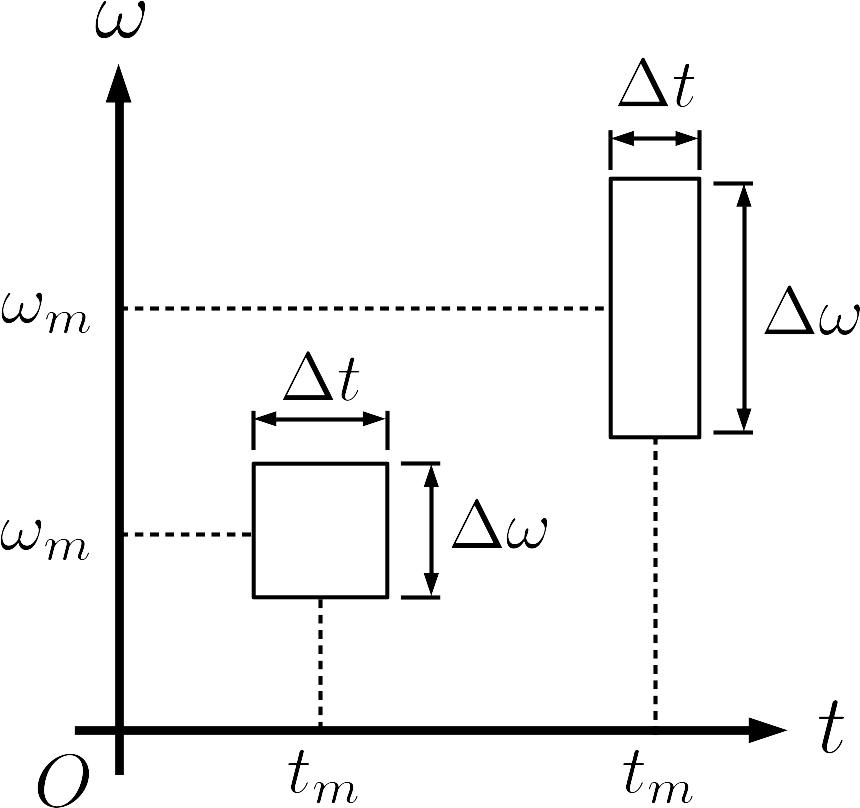
\includegraphics[width=60mm]{./figs/heisenburg_box.png}
    \end{figure}
    この図に現れる矩形領域をハイゼンベルクの箱と言う.
\end{frame}

\subsection{不確定性原理の証明} 

\begin{frame}[c]
    \frametitle{不確定性原理の証明}
    \scriptsize
    $g(t) = \exp(-j\omega_{m}t) f(t + t_{m})$とおく.$g(t)$のフーリエ変換$G(\omega)$は,
    \begin{align*}
        G(\omega) &= \int^{\infty}_{-\infty} g(t) \exp(-j\omega t) \mathrm{d}t \\
        &= \int^{\infty}_{-\infty} f(t + t_{m}) \exp[-j(\omega + \omega_{m}) t] \mathrm{d}t \\
        &= \exp[-j(\omega + \omega_{m}) t_{m}] \int^{\infty}_{-\infty} f(t + t_{m}) \exp[-j(\omega + \omega_{m}) (t + t_{m})] \mathrm{d}t \\
        &= \exp[-j(\omega + \omega_{m}) t_{m}] F(\omega + \omega_{m})
    \end{align*}
    このとき,
    \begin{align*}
        & \left\{ \int_{-\infty}^{\infty} (t - t_{m})^{2} |f(t)|^{2} \mathrm{d}t \right\} \left\{ \frac{1}{2\pi} \int_{-\infty}^{\infty} (\omega - \omega_{m})^{2} |F(\omega)|^{2} \mathrm{d}\omega \right\} \\
        &= \left\{ \int_{-\infty}^{\infty} s^{2} |f(s + t_{m})|^{2} \mathrm{d}s \right\} \left\{ \frac{1}{2\pi} \int_{-\infty}^{\infty} u^{2} |F(u + \omega_{m})|^{2} \mathrm{d}u \right\} \\
        &= \left\{ \int_{-\infty}^{\infty} s^{2} |\exp(j\omega_{m}s)g(s)|^{2} \mathrm{d}s \right\} \left\{ \frac{1}{2\pi} \int_{-\infty}^{\infty} u^{2} |\exp[-j(u+\omega_{m})t_{m}]G(u)|^{2} \mathrm{d}u \right\} \\
        &= \left\{ \int_{-\infty}^{\infty} s^{2} |g(s)|^{2} \mathrm{d}s \right\} \left\{ \frac{1}{2\pi} \int_{-\infty}^{\infty} u^{2} |G(u)|^{2} \mathrm{d}u \right\} \quad (\because {}^{\forall} x \in \mathbb{R}.\ |\exp(jx)| = 1)
    \end{align*}
    だから,$t_{m} = \omega_{m} = 0$として考える.
\end{frame}

\begin{frame}[c]
    \frametitle{不確定性原理の証明}
    \scriptsize
    また,
    \begin{align*}
        f^{\prime}(t) &= \difrac{}{t} \left\{ \frac{1}{2\pi} \int^{\infty}_{-\infty} F(\omega) \exp(j\omega t) \mathrm{d}t \right\} \\
        &= \frac{1}{2\pi} \int^{\infty}_{-\infty} F(\omega) \difrac{}{t} \exp(j\omega t) \mathrm{d}t \quad \text{(順序交換可能とする)} \\
        &= \frac{j\omega}{2\pi} \int^{\infty}_{-\infty} F(\omega) \exp(j\omega t) \mathrm{d}t \\
        &= j\omega f(t)
    \end{align*}
    より,以下の関係式が得られる.
    \begin{align*}
        \ft{f^{\prime}(t)} &= j\omega\ft{f(t)} = j\omega F(\omega) \\
        \implies \left| \ft{f^{\prime}(t)} \right|^{2} &= \omega^{2} |F(\omega)|^{2}
    \end{align*}
    これより,
    \begin{align*}
        \frac{1}{2\pi} \int_{-\infty}^{\infty} \omega^{2} |F(\omega)|^{2} \mathrm{d}\omega &= \frac{1}{2\pi} \int_{-\infty}^{\infty} \left| \ft{f^{\prime}(t)}\right|^{2} \mathrm{d}\omega \\
        &= \int_{-\infty}^{\infty} |f^{\prime}(t)|^{2} \mathrm{d}t \quad \text{($\because$ パーセバルの等式)}
    \end{align*}
\end{frame}

\begin{frame}[c]
    \frametitle{不確定性原理の証明}
    \scriptsize
    不等式左辺($=(\Delta t)^{2}(\Delta \omega)^{2}$)を変形していくと,
    \begin{align*}
        & \left\{ \int_{-\infty}^{\infty} t^{2} |f(t)|^{2} \mathrm{d}t \right\} \left\{ \frac{1}{2\pi} \int_{-\infty}^{\infty} \omega^{2} |F(\omega)|^{2} \mathrm{d}u \right\} = \left\{ \int_{-\infty}^{\infty} t^{2} |f(t)|^{2} \mathrm{d}t \right\} \left\{ \int_{-\infty}^{\infty} |f^{\prime}(t)|^{2} \mathrm{d}u \right\} \\
        &\geq \int_{-\infty}^{\infty} \left| t f(t) f^{\prime}(t) \right|^{2} \mathrm{d}t \quad \text{($\because$ シュワルツの不等式$\norm{\ve{v}}{2}\norm{\ve{w}}{2} \geq \norm{\innprod{\ve{v}}{\ve{w}}}{2}$)} \\
        &\geq \frac{1}{4} \int_{-\infty}^{\infty} \left\{ t f(t) \roverline{f^{\prime}(t)} + t \roverline{f(t)} f^{\prime}(t) \right\}^{2} \mathrm{d}t \quad (\because |ab| \geq \frac{1}{2} |a\roverline{b} + \roverline{a}b|) \\
        &\geq \frac{1}{4} \left[ \int_{-\infty}^{\infty} \left\{ t f(t) \roverline{f^{\prime}(t)} + t \roverline{f(t)} f^{\prime}(t) \right\} \mathrm{d}t \right]^{2} \\
        &= \frac{1}{4} \left[ \int_{-\infty}^{\infty} t \difrac{}{t} \left\{ f(t) \roverline{f(t)} \right\} \mathrm{d}t \right]^{2} \quad \text{($\because$ 積の微分公式)} \\
        &= \frac{1}{4} \left\{ \left[ t |f(t)|^{2} \right]_{-\infty}^{\infty} - \int_{-\infty}^{\infty} |f(t)|^{2} \mathrm{d}t \right\}^{2} \quad \text{($\because$ 部分積分と$f(t) \roverline{f(t)} = |f(t)|^{2}$)} \\
        &= \frac{1}{4} \left\{ 0 - 1 \right\}^{2} \quad \text{($\because$ $f(t)$に関する仮定)} \\
        &= \frac{1}{4} 
    \end{align*}
    よって不確定性原理は示された.
\end{frame}

\section{フーリエ変換における諸性質}

\subsection{様々なパーセバルの等式}

\begin{frame}[c]
    \frametitle{パーセバルの等式\small(フーリエ級数)}
    \scriptsize
    周期$2\pi$の関数$f(x), g(x)$をそれぞれ以下のようにフーリエ級数展開できるとする:
    \begin{align*}
        f(x) &= \sum_{n} c_{n} \exp(j\omega x), \ c_{n} = \frac{1}{2\pi} \int_{-\pi}^{\pi} f(x) \exp(-jn\omega) \mathrm{d} x \\
        g(x) &= \sum_{n} d_{n} \exp(j\omega x), \ d_{n} = \frac{1}{2\pi} \int_{-\pi}^{\pi} g(x) \exp(-jn\omega) \mathrm{d} x
    \end{align*}
    このとき,
    \begin{align*}
        \int_{-\pi}^{\pi} f(x) \roverline{g(x)} \mathrm{d} x &= \int_{-\pi}^{\pi} \left\{ \sum_{n} c_{n} \exp(j\omega x) \right\} \roverline{g(x)} \mathrm{d} x \\
        &= \sum_{n} c_{n} \int_{-\pi}^{\pi} \roverline{g(x)} \exp(jnx) \mathrm{d} x = \sum_{n} c_{n} \roverline{\int_{-\pi}^{\pi} g(x) \exp(-jnx) \mathrm{d} x} \\
        &= 2\pi \sum_{n} c_{n} \roverline{d_{n}}
    \end{align*}
    が成立する.とくに$f=g$とすれば,
    \begin{align*}
        \int_{-\pi}^{\pi} |f(x)|^{2} \mathrm{d} x = 2\pi \sum_{n} |c_{n}|^{2}
    \end{align*}
\end{frame}

\begin{frame}[c]
    \frametitle{パーセバルの等式\small(フーリエ変換)}
    \scriptsize
    関数$f(x), g(x)$のフーリエ変換対を以下のように書く:
    \begin{align*}
        F(\omega) &= \int_{-\infty}^{\infty} f(x) \exp(-j\omega x) \mathrm{d} x,\ f(x) = \frac{1}{2\pi} \int_{-\infty}^{\infty} F(\omega) \exp(j\omega x) \mathrm{d} \omega \\
        G(\omega) &= \int_{-\infty}^{\infty} g(x) \exp(-j\omega x) \mathrm{d} x,\ g(x) = \frac{1}{2\pi} \int_{-\infty}^{\infty} G(\omega) \exp(j\omega x) \mathrm{d} \omega
    \end{align*}
    このとき,
    \begin{align*}
        \int_{-\infty}^{\infty} f(x) \roverline{g(x)} \mathrm{d} x &= \int_{-\infty}^{\infty} \left\{ \frac{1}{2\pi} \int_{-\infty}^{\infty} F(\omega) \exp(j\omega x) \mathrm{d} \omega \right\} \roverline{g(x)} \mathrm{d} x \\
        &= \frac{1}{2\pi} \int_{-\infty}^{\infty} F(\omega) \left\{ \int_{-\infty}^{\infty} \roverline{g(x)} \exp(j\omega x) \mathrm{d} x \right\} \mathrm{d} \omega \\
        &= \frac{1}{2\pi} \int_{-\infty}^{\infty} F(\omega) \left\{ \roverline{\int_{-\infty}^{\infty} g(x) \exp(-j\omega x) \mathrm{d} x} \right\} \mathrm{d} \omega \\
        &= \frac{1}{2\pi} \int_{-\infty}^{\infty} F(\omega) \roverline{G(\omega)} \mathrm{d} \omega
    \end{align*}
    が成立する.とくに$f=g$とすれば,
    \begin{align*}
        \int_{-\infty}^{\infty} |f(x)|^{2} \mathrm{d} x &= \frac{1}{2\pi} \int_{-\infty}^{\infty} |F(\omega)|^{2} \mathrm{d} \omega
    \end{align*}
\end{frame}

\begin{frame}[c]
    \frametitle{パーセバルの等式\small(高速ウェーブレット変換)}
    \begin{mylemma}[パーセバルの等式]
        高速ウェーブレット変換の列$\{p_{m+1}[n]\}$,$\{p_{m}[n]\}$,$\{q_{m}[n]\}$に関して次が成立する:
        \begin{align}
            \norm{p_{m+1}}{2}^{2} = \norm{p_{m}}{2}^{2} + \norm{q_{m}}{2}^{2}
        \end{align}
    \end{mylemma}
    入力信号のエネルギー$\norm{p_{m+1}}{2}^{2}$は$\norm{p_{m}}{2}^{2}$と$\norm{q_{m}}{2}^{2}$に分配される.
\end{frame}

\begin{frame}[c]
    \frametitle{パーセバルの等式\small(高速ウェーブレット変換)}
    \scriptsize
    (証明)式\eqref{eq:mra_downsampling}の両辺のノルムをとると,
    \begin{align*}
        \left|\left|
            \left[\begin{array}{c}
                P_{m}(\omega) \\
                Q_{m}(\omega)
            \end{array}\right]
        \right|\right|_{2}^{2}
        &=
        \frac{1}{2}
        \left|\left|
        \ve{H}\left(\frac{\omega}{2}\right)
            \left[\begin{array}{c}
                P_{m+1}\left(\frac{\omega}{2}\right) \\
                P_{m+1}\left(\frac{\omega}{2} + \pi\right)
            \end{array}\right] 
        \right|\right|_{2}^{2} \\
        &=
        \frac{1}{2}
        \left|\left|
            \left[\begin{array}{c}
                P_{m+1}\left(\frac{\omega}{2}\right) \\
                P_{m+1}\left(\frac{\omega}{2} + \pi\right)
            \end{array}\right] 
        \right|\right|_{2}^{2}  \quad \text{($\because$ $\ve{H}(\omega)$はユニタリ行列)} \\
        \iff |P_{m}(\omega)|^{2} + |Q_{m}(\omega)|^{2} &= \frac{1}{2} \left\{ \left|P_{m+1}\left(\frac{\omega}{2}\right)\right|^{2} + \left|P_{m+1}\left(\frac{\omega}{2} + \pi\right)\right|^{2} \right\}
    \end{align*}
    離散時間フーリエ変換のパーセバルの等式により,
    \begin{align*}
        \norm{p_{m}}{2}^{2} + \norm{q_{m}}{2}^{2} &= \frac{1}{2\pi} \int_{-\pi}^{\pi} \left( |P_{m}(\omega)|^{2} + |Q_{m}(\omega)|^{2} \right) \mathrm{d} \omega \\
        &= \frac{1}{4\pi} \int_{-\pi}^{\pi} \left\{ \left|P_{m+1}\left(\frac{\omega}{2}\right)\right|^{2} + \left|P_{m+1}\left(\frac{\omega}{2} + \pi\right)\right|^{2} \right\} \mathrm{d} \omega \\
        &= \frac{1}{2\pi} \int_{-\frac{\pi}{2}}^{\frac{\pi}{2}} \left\{ |P_{m+1}(s)|^{2} + |P_{m+1}(s + \pi)|^{2} \right\} \mathrm{d} s \quad (\omega = 2s) \\
        &= \frac{1}{2\pi} \int_{-\frac{\pi}{2}}^{\frac{3}{2}\pi} |P_{m+1}(s)|^{2} \mathrm{d} s = \frac{1}{2\pi} \int_{-\pi}^{\pi} |P_{m+1}(s)|^{2} \mathrm{d} s \\
        &= \norm{p_{m+1}}{2}^{2}
    \end{align*}
\end{frame}

\subsection{間引いた数列の離散時間フーリエ変換}

\begin{frame}[c]
    \frametitle{間引いた数列の離散時間フーリエ変換}
    \begin{mylemma}[間引いた数列の離散時間フーリエ変換]
        $x[n]$の離散時間フーリエ変換を$X(\omega)$と書く.$x[n]$のサンプリング間隔を$D$倍に間引いた数列の離散時間フーリエ変換は,
        \begin{align}
            \frac{1}{D} \sum_{k = 0}^{D - 1} X\left( \frac{\omega - 2\pi k}{D} \right) \label{eq:decimated_dtft} 
        \end{align}
    \end{mylemma}
\end{frame}

\begin{frame}[c]
    \frametitle{間引いた数列の離散時間フーリエ変換}
    \scriptsize
    (証明)間引き操作は,$x[n]$に周期$D$のインパルス関数列
    \begin{align*}
        \delta_{D}[n] &:= 
        \left\{
            \begin{array}{cl}
                1 & \text{$n$が$D$の倍数} \\
                0 & \text{otherwise}
            \end{array}
        \right. \\
        &= \frac{1}{D} \sum_{k = 0}^{D - 1} \exp\left( j \frac{2\pi nk}{D} \right) \quad \text{($\because$ 証明は次のページ)}
    \end{align*}
    を乗じてから,$D$個おきの出力を得る操作($y[n]:=x[n]\delta_{D}[n]$として$y[Dn]$が結果)と解釈できる.
    $y[Dn]$を離散時間フーリエ変換すると,
    \begin{align*}
        \ft{y[Dn]} &= \sum_{n} y[Dn] \exp(-jn\omega) = \sum_{n} y[n] \exp\left(-j\frac{n\omega}{D}\right) \\
        &= \sum_{n} x[n]\delta_{D}[n] \exp\left(-j\frac{n\omega}{D}\right) \\
        &= \frac{1}{D} \sum_{k = 0}^{D - 1} \sum_{n} x[n] \exp\left( j \frac{2\pi nk}{D} - j\frac{n\omega}{D} \right) \quad \text{($\because$ 式\eqref{eq:decimated_impulse_seq})}\\
        &= \frac{1}{D} \sum_{k = 0}^{D - 1} \sum_{n} x[n] \exp\left( -jn \frac{\omega - 2\pi k}{D} \right) \\
        &= \frac{1}{D} \sum_{k = 0}^{D - 1} X\left( \frac{\omega - 2\pi k}{D} \right)
    \end{align*} 
\end{frame}

\begin{frame}[c]
    \frametitle{間引いた数列の離散時間フーリエ変換}
    \scriptsize
    \begin{block}{}
    \vspace*{-17pt}
    \begin{align}
        \delta_{D}[n] = \frac{1}{D} \sum_{k = 0}^{D - 1} \exp\left( j \frac{2\pi nk}{D} \right) \label{eq:decimated_impulse_seq}
    \end{align}
    \end{block}
    (証明)$n$が$D$の倍数のときは$n = mD\ (m \in \mathbb{Z})$と書けるから,
    \begin{align*}
        \frac{1}{D} \sum_{k = 0}^{D - 1} \exp\left( j \frac{2\pi nk}{D} \right) = \frac{1}{D} \sum_{k = 0}^{D - 1} \exp( j 2\pi mk ) = \frac{1}{D} \sum_{k = 0}^{D - 1} 1 = 1
    \end{align*}
    \\~\
    $n$が$D$の倍数ではないときは$\displaystyle W_{k} := \exp\left(j\frac{2\pi nk}{D}\right)$とおくと,$(W_{k})^{D} = \exp(j2\pi nk) = 1$より,$W_{k}\ (k = 0,1, ..., D-1)$は$1$の$D$乗根,すなわち,方程式$x^{D} - 1 = 0$の解となっている.方程式左辺を因数分解すると,
    \begin{align*}
        x^{D} - 1 &= (x - W_{0})(x - W_{1})...(x - W_{D-1}) \\
        &= x^{D} - (W_{0} + W_{1} + ... + W_{D-1}) x^{D-1} + ... + (-1)^{D}W_{0}W_{1}...W_{D-1}
    \end{align*} 
    両辺の係数を比較する.$x^{D-1}$の係数は$0$だから,
    \begin{align*}
        W_{0} + W_{1} + ... + W_{D-1} = \sum_{k = 0}^{D-1} W_{k} = \sum_{k = 0}^{D-1} \exp\left(j\frac{2\pi nk}{D}\right) = 0
    \end{align*} 
\end{frame}

\section{参考文献}

\begin{frame}[c]
  \frametitle{参考資料の概観}
  \footnotesize
  webで入手できる資料:
  \begin{itemize}
  \item \cite{ito_wavelet, haneishi_wavelet1, haneishi_wavelet2} 大学講義資料.取っ掛かりに.
  \item \cite{fussy_wavelet1, fussy_wavelet2} 分かりやすい.C++ソース解説も充実.
  \item \cite{ian_lifting} Liftingの簡易な説明.ソースもある.
  \item \cite{fujinoki2014, uytterhoeven1997, fujinoki2018} Liftingの資料.とくに\cite{uytterhoeven1997}は簡明.
  \end{itemize}
  書籍:
  \begin{itemize}
  \item \cite{kanatani2003} 分かりやすい.ただしハールウェーブレットのみ.
  \item \cite{nakano_wavelet} 分かりやすい.C言語ソースあり.
  \item \cite{toda2005} 分かりやすいが絶版...C++ソースあり.
  \item \cite{hubbard2003} 歴史を概観するのに適する.意外に理論も深い.
  \item \cite{maeda2001} 一番参考にした.信号処理から見た解説も秀逸.
  \item \cite{daubechies2012} ドベシィ様執筆.基礎理論を網羅.読みきれてない.
  \item \cite{chui1993} 関数解析必須.(挫折)
  \end{itemize}
\end{frame}

\begin{frame}[allowframebreaks]{参考文献}
\scriptsize
\beamertemplatetextbibitems
\printbibliography[heading=none]
\end{frame}

\end{document}
